\documentclass[a4paper,10pt]{article}
\usepackage{ifpdf}

\ifpdf
\usepackage[pdftex]{graphicx}
\usepackage[pdftex]{hyperref}
\else
\usepackage{graphicx}
\usepackage{hyperref}
\fi

\usepackage[svgnames]{xcolor}
\usepackage{minted}
\usepackage{amsmath}
\usepackage{amssymb}
\usepackage{xspace}
\usepackage{booktabs}
\usepackage{pifont}
\usepackage{longtable}
\usepackage[top=3cm, bottom=3cm, left=2.5cm,right=2.5cm]{geometry}
%\usepackage[left=3cm,right=3cm]{geometry}

\pagestyle{headings}

\author{Stuart Moodie}
\date{August 29, 2013}
\title{Record of changes added to version 0.2.0 of \pharmml}

\colorlet{bkgd}{gray!5}
%\usemintedstyle{trac}

%\newminted{xml}{bgcolor=bkgd,fontsize=\footnotesize%
%,fontfamily=courier%
%}

\newminted{xml}{fontsize=\footnotesize,fontfamily=courier}

% \newcommand{\inputxml}[1]{\inputminted[bgcolor=bkgd,fontsize=\scriptsize%
% ,fontfamily=courier%
% ]{xml}{codesnippets/#1}}

\newcommand{\cellml}{CellML\xspace}
\newcommand{\sbml}{SBML\xspace}
\newcommand{\sedml}{SED-ML\xspace}
\newcommand{\mathml}{MathML\xspace}
\newcommand{\uncertml}{UncertML\xspace}
\newcommand{\pharmml}{PharmML\xspace}
\newcommand{\xelem}[1]{\texttt{<#1>}\index{XML Element!\texttt{<#1>}}}
\newcommand{\xatt}[1]{\texttt{#1}\index{XML Attribute!\texttt{#1}}}
\reversemarginpar  % Want "\watchout" to be put on the left, not the right.
\newcommand{\watchout}{\marginpar{\hspace*{34pt}\raisebox{-0.5ex}{\Large\ding{43}}}}

\begin{document}

\maketitle

\tableofcontents

\section{Introduction}

I want us to be clear what will be in \pharmml version~0.2.0. I've
written up all the changes and new features that I have incorporated
into the XML Schema and thus which I think will go in the language
specification. To do this I've taken the content of the previous
proposal docs and extracted those changes that were agreed upon. In
some cases the initial proposal has been modified based on review
comments and other input. In such cases I have highlighted parts that
have changed with the \watchout\emph{take note} symbol that you see in
the left margin.

Note that all items have been implemented in the XML schema except
the Unresolved Issues in section~\ref{sec:unresolved-issues}.

\section{New changes not fully reviewed}

\subsection{Cleaning up symbol definitions and scopes}

With the trial design changes (see section
\ref{sec:trialdesignchanges}) we have effectively created a new class
of identifier in PharmML, the \emph{object} identifier. This is
borrowed from CDISC XML where they use the attribute \xatt{oid} to
identify and to reference components used in the design. In \pharmml
we exclusively the Object identifier to identify components in the
Trial Design and Modelling Steps sections of a \pharmml
document. Symbol identifier are exclusively used to identify
paramaters and variables within the ModelDefinition section.

Object identifiers have global scope, which contrasts with the global
scope for symbol identifiers. Note also that the block identifiers
used to identify elements such as the \xelem{ParameterModel} in the
Model Definition are \emph{not} Object Identifiers. For consistency I
have adopted an attribute naming convention that distinguishes between
definitions and references by appending \texttt{Ref} to all such
attribute names. As in these code snippets:
%
\begin{xmlcode}
<ct:VariableAssignment>
    <ct:SymbRef blkIdRef="p1" symbIdRef="pop_IC50"/>
    <ct:Assign>
        <ct:Real>0.4</ct:Real>
    </ct:Assign>
</ct:VariableAssignment>

<Cell oid="c2">
    <EpochRef oidRef="e1" />
    <ArmRef oidRef="a2"/>
    <SegmentRef oidRef="tb"/>
</Cell>
\end{xmlcode}

As a consequence we will change the scoping rules of the
language. Identifiers defined using the attribute \xatt{symbId} will
be known as Symbol identifiers and those defined by \xatt{oid} will be
know as Object identifiers. The rules applied to them are asd follows:
%
\begin{itemize}
\item Symbol identifier scoping is as before with block and symbol
  identifiers and the same referencing rules. Note however, that
  symbol references can only point to symbols not to Objects.
\item Object identifiers have global scope. All such symbols must be
  unique within the \pharmml document. References to objected
  identifiers (using the \xatt{oidRef} attribute) must only refer to
  Object identifiers.
\item Symbol block identifiers (\xatt{blkId}) and Object identifiers
  (\xatt{oid}) share the same namespace so the union of both
  identifier sets must be unique.
\end{itemize}

\subsection{Symbol Definition Refactored}

The current definition of \xelem{SymbolDefinition} needs tidying
up. The SymbolDefinition is now really a mechanism for defining
functions while originally I had the idea of using it to define
constants and there was a parallel element that referred to an
external definition of symbols and functions. Therefore, it makes
sense to rename it to \xelem{FunctionDefinition} and to reorganise it
slightly. The current version looks like this:
%
\begin{xmlcode}
<SymbolDefinition symbId="constantErrorModel" symbolType="scalar">
    <FunctionDefinition>
        <FunctionArgument symbId="a" symbolType="scalar"/>
        <Definition>
            <Equation xmlns="http://www.pharmml.org/2013/03/Maths" writtenVersion="0.1">
                <Var symbIdRef="a"/>
            </Equation>
        </Definition>
    </FunctionDefinition>
</SymbolDefinition>
\end{xmlcode}
%
I propose to restructure it so that it looks like this:
%
\begin{xmlcode}
<FunctionDefinition xmlns="http://www.pharmml.org/2013/03/CommonTypes"
    symbId="constantErrorModel" symbolType="real">
    <FunctionArgument symbId="a" symbolType="real"/>
    <Definition>
        <Equation xmlns="http://www.pharmml.org/2013/03/Maths" writtenVersion="0.1">
            <Var symbIdRef="a"/>
        </Equation>
    </Definition>
</FunctionDefinition>
\end{xmlcode}
%
As well as renaming it I propose to move the definition into the
common types schema. It is currently in the top-level pharmML schema.
  
\subsubsection*{Conclusion}

Added to schema.

\subsection{Initial Conditions}

In version 0.1 of the \pharmml specification and in the previous
proposal we do not clearly define what we mean by the initial
condition of a derivative variable. While we set the value for each
derivative we did not specify the time. I've discussed this with
Maciej and he strongly feels that we need to specify the time of the
initial condition. I was initially persuaded but after some reflection
I don't think we need to change the current approach.


Looking at SBML they do not specify a time for the initial
condition. The SBML specification discusses initial conditions in
terms of simulation and they assume that such initial conditions are
set at the start of the simulation. This is consistent with version
0.1 of the \pharmml specification.

To understand the problem with setting the time of the initial
condition it is useful to consider how you might use a model where the
initial condition time is set explicitly. For example, given the
following system of ODEs, where $ \mathrm{Ad}_{\mathrm{init}}$ is an
arbitrary non-zero quantity:
%
\begin{align*}
k&=\frac{\mathrm{CL}}{V} \\
\frac{d\mathrm{Ad}}{dt} &=-\mathrm{ka} \, \mathrm{Ad}  \\
\frac{d\mathrm{Ac}}{dt}&=\mathrm{ka} \, \mathrm{Ad} - k \, \mathrm{Ac}  \\
\frac{dE}{dt} &=\mathrm{Rin} \Bigg(1-\frac{\mathrm{Imax} \mathrm{Cc}}{\mathrm{Cc}+\mathrm{IC50}}\Bigg)
- \mathrm{kout} E \\
\mathrm{Cc} &= \frac{\mathrm{Ac}}{V} 
\intertext{initial conditions:}
E(t=2) &= \frac{\mathrm{Rin}}{\mathrm{kout}}\\
\mathrm{Ad}(t=2) &= \mathrm{Ad}_{\mathrm{init}}  \\
\mathrm{Ac}(t=2) &=0
\end{align*}
%
let's assume we simulate or estimate a model based on this structural
model. If the first observation time given is $t=2$ then these are
clearly initial conditions. However, what if we specify a bolus dose
at $t=1$?  The simulation or estimation task must then start at $t=1$
and we have two problems. First at $t=1$ we have no initial condition
set for the above ODEs and second what does $\mathrm{Ac}(t=2) =
D$ now mean? It is not an input into the system. Perhaps we should try and
infer from it what the value of $Ac(t=1)$ is? But is that what the
author of the model intended us to do? Perhaps there is a mistake and
he meant the first dose to start at $t=2$?

Take another example. Say the first bolus dose is given at $t=20$ and
the first observation time is t=$25$. When does the simulation or
estimation start?  Ordinarily I would say at $t=20$, but because the
time of the initial condition is $t=2$ should it start then?

We could constrain this by stating that the simulation or estimation
cannot start dosing or have an observation before the time of the
initial condition, but I think this is bad design. It means that the
ModelDefinition is in effect defining the start of the estimation or
simulation step, which goes against our design principles. We have
always aimed to allow the ModelDesign to be reusable by different
tasks within the same \pharmml document. But by specifying the initial
condition time in the model we restrict the possible dosing and
observation times in the model.

We have always aimed to design \pharmml to be as simple as it can be,
with as few rules as it needs --- the principle of parsimony. Applying
a rule that an initial condition value specified in the \pharmml
document is applied at the beginning of the estimation or simulation
task satisfies the above and will compatible with tools using
\pharmml. In this case not changing the XML is the best course to
take, we should just clarify our definition in the specification doc.

\subsection{Revised dataset}
\label{sec:dataset-refactoring}

I've made a number of changes to the dataset from the previous release
of \pharmml. These changes have aimed to:
\begin{enumerate}
\item improve the typing of the data held in the table,
\item support for a null type,
\item support only XML formatted data (other formats are no longer
  supported),
\item clarify its semantics,
\item only support `inline' data. Linking of external data is removed
  (for now).
\end{enumerate}
%
In this way the dataset is simpler (it uses only of XML to define
data) and more clearly defined. By making sure that data is only held
in the \pharmml document we are making it simpler to use and validate
it (see section \ref{sec:no-ext-res}). Below is an example of a basic
data-set:
%
\begin{xmlcode}
<ds:DataSet>
    <ds:Definition>
        <ds:Column columnId="id" valueType="string" columnNum="1"/>
        <ds:Column columnId="arm" valueType="string" columnNum="2"/>
        <ds:Column columnId="reps" valueType="int" columnNum="3"/>
    </ds:Definition>
    <ds:Table>
        <ds:Row>
            <ct:String>i1</ct:String><ct:String>a1</ct:String><ct:Int>20</ct:Int>
        </ds:Row>
        <ds:Row>
            <ct:String>i2</ct:String><ct:String>a2</ct:String><ct:Int>20</ct:Int>
        </ds:Row>
        <ds:Row>
            <ct:String>i3</ct:String><ct:String>a3</ct:String><ct:Int>40</ct:Int>
        </ds:Row>
        <ds:Row>
            <ct:String>i4</ct:String><ct:String>a4</ct:String><ct:Int>40</ct:Int>
        </ds:Row>
    </ds:Table>
</ds:DataSet>
\end{xmlcode}
%
As before the dataset has a definition, where the columns of the
dataset table are defined. The column number must start at 1 and each
column must be numbered in consecutive order (i.e.,\xspace
1,2,3,4\ldots etc.). The type of each column is specified and this
complies with the \pharmml type system.  Next the content of the
dataset is held within the \xelem{Table} element and this consists of
one or more \xelem{Row} elements. Each row must contain an entry for
each column defined. NULL values are indicated by the \xelem{Null/}
element. 

This looks like a table in a relational database and indeed this
approach is based on the concept of a relation in relational
theory. Therefore the ordering of rows is not significant. At present
there is no mechanism to define a key on the dataset or columns that
cannot be NULL. It is assumed such restrictions may be applied when
the dataset is used. For example it is assumed that when mapping
objective data in the \xelem{EstimationStep} that none of the data is
NULL and that the combination of the time column and that identifying
the individual are unique.

\begin{figure}[htb]
\centering
%\setlength\fboxsep{0pt}
%\setlength\fboxrule{0.5pt}
%\fbox{%
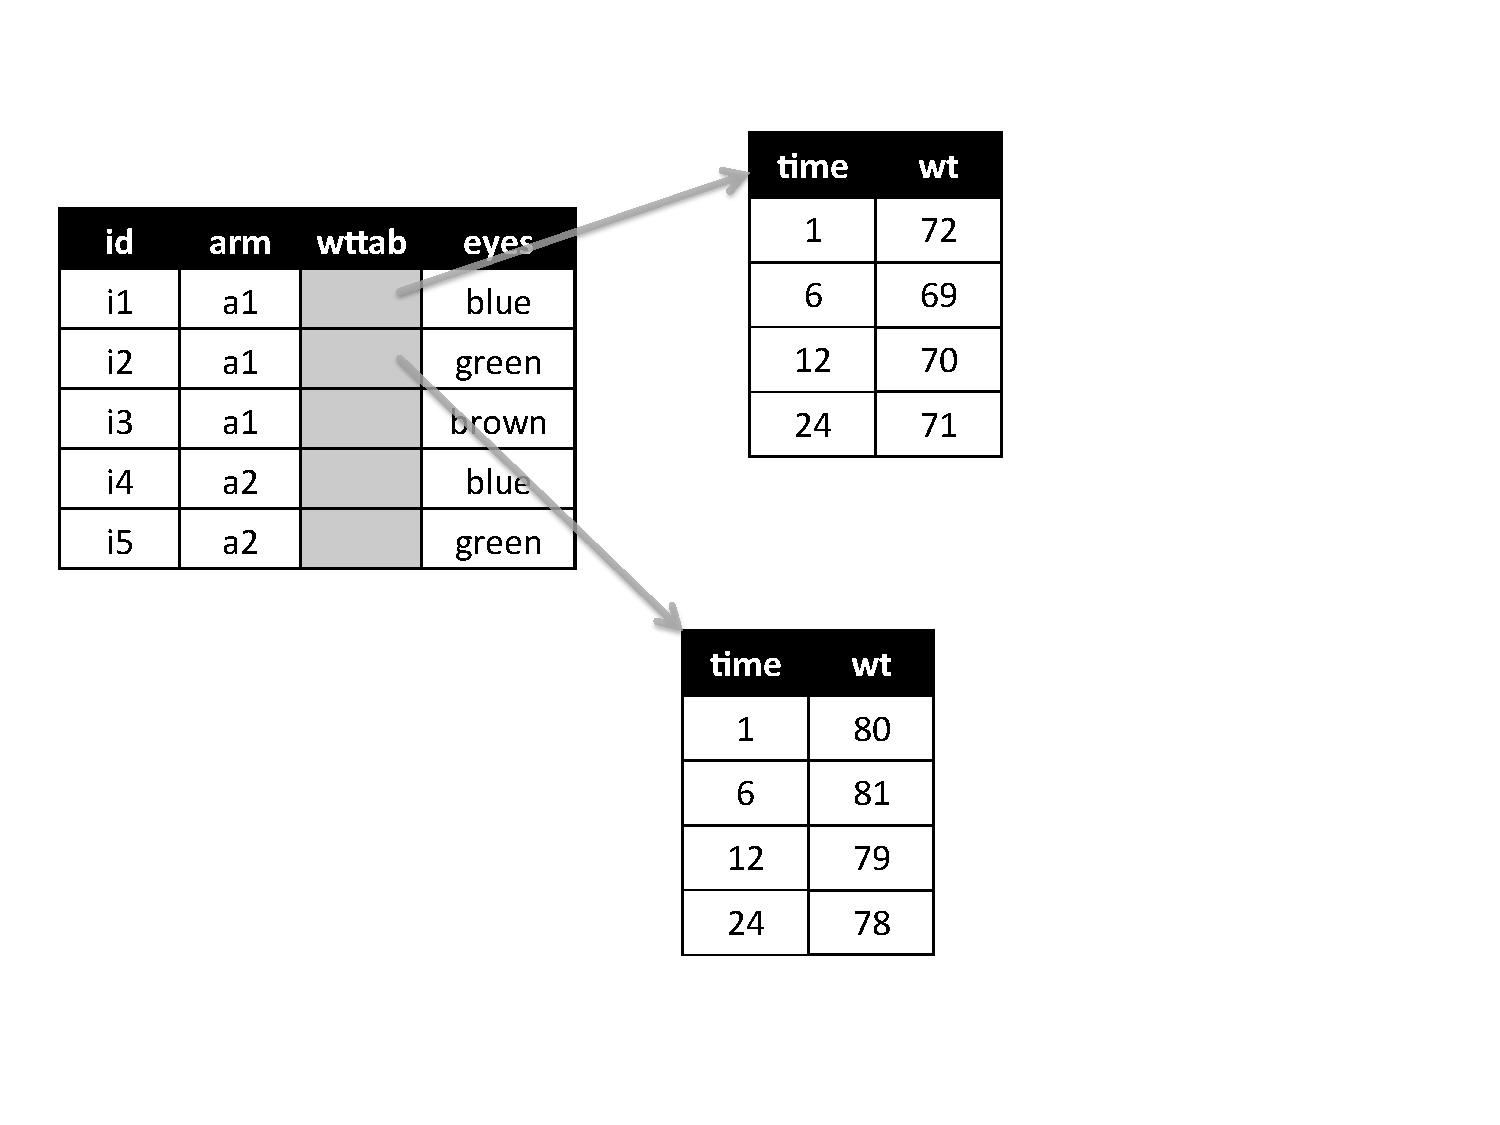
\includegraphics[height=0.35\textheight,clip=true,trim=9mm 1.5cm 8.3cm 2cm]{Datasets}%
%}
\caption{An illustration of how a table with a nested table can be
  conceptualised. Each cell within the \xatt{wttab} column contains
  another table.}
\label{fig:dataset}
\end{figure}

 Finally, there is one deviation from standard relational theory in the
dataset. This is that a table can be nested multiple times, i.e., a
table can contain a column that is another table and so on. This
concept is illustrated in figure \ref{fig:dataset}. This is required
because in some situations it is necessary to define one to many
relationships within the data. For example when defining a population
of individuals in a study whose weight changes during the course of
the study (weight is a time-dependent covariate). In relational theory
this is achieved by a foreign key relationship, but in the dataset is
it simpler and clearer if we take advantage of the hierarchical nature
of the XML. You can see this in the example dataset below:
%
\begin{xmlcode}
<ds:DataSet>
    <ds:Definition>
        <ds:Column columnId="id" valueType="string" columnNum="1"/>
        <ds:Column columnId="arm" valueType="string" columnNum="2"/>
        <ds:Table tableId="wttab">
            <ds:Column columnId="epoch" valueType="string" columnNum="1"/>
            <ds:Column columnId="wt" valueType="real" columnNum="2"/>
        </ds:Table>
    </ds:Definition>
    <ds:Table>
        <ds:Row>
            <ct:String>i552</ct:String><ct:String>a1</ct:String>
                <ds:Table>
                    <ds:Row><ct:String>m1</ct:String><ct:Real>73</ct:Real></ds:Row>
                    <ds:Row><ct:String>m6</ct:String><ct:Real>70</ct:Real></ds:Row>
                    <ds:Row><ct:String>m12</ct:String><ct:Real>73</ct:Real></ds:Row>
                    <ds:Row><ct:String>m24</ct:String><ct:Real>71</ct:Real></ds:Row>
                    <ds:Row><ct:String>m48</ct:String><ct:Real>69</ct:Real></ds:Row>
                </ds:Table>
        </ds:Row>
        <ds:Row>
            <ct:String>i553</ct:String><ct:String>a1</ct:String>
            <ds:Table>
                <ds:Row><ct:String>m1</ct:String><ct:Real>75</ct:Real></ds:Row>
                <ds:Row><ct:String>m6</ct:String><ct:Real>74</ct:Real></ds:Row>
                <ds:Row><ct:String>m12</ct:String><ct:Real>75</ct:Real></ds:Row>
                <ds:Row><ct:String>m24</ct:String><ct:Real>72</ct:Real></ds:Row>
                <ds:Row><ct:String>m48</ct:String><ct:Real>70</ct:Real></ds:Row>
            </ds:Table>
        </ds:Row>
    </ds:Table>
</ds:DataSet>
\end{xmlcode}
%
In the example the child table is defined by using a \xelem{Table}
element instead of the usual \xelem{Column} element and given the identifier
``wttab''. Within the nested table definition another set of
columns is specified\footnote{Of course this definition can itself
  contain another table definition \emph{ad infinitum}.} as you would
expect. Now when encoding the data within the dataset the rows of the
dataset are defined as before, but where a column has been replaced by
a nested table the contents of this table are delimited by an
\xelem{Table} element. The dataset in the example defines
individual \texttt{i552} assigned to arm \texttt{a1} with a weight
that varies between $69$ and $73 kg$ during the five epochs of the
study.

\subsection{No external inclusions}
\label{sec:no-ext-res}

We have discussed not including external SBML models (see section
\ref{sec:include-sbml}), but I am proposing we take this to its
natural conclusion and remove the inclusions of data and other models
completely. I'm not suggesting that we do this permanently, but
instead we to do this for version 0.2.0 and reintroduce this
functionality later. Why?  Mainly for the sake of
simplicity. Inclusion makes the XML definition and rules more
complicated, the validation more complication and the development of
supporting software more complicated. \pharmml will be very
complex as it is and so the challenges of validating it will be
considerable. This approach is essentially one of \emph{Divide and
  Conquer}: implement support for \pharmml without inclusions first
and then extend existing implementations to support inclusion of
external resources once we have this working.

\subsection{Repeating a simulation}

In version 0.1 of \pharmml we could specify that a simulation be
repeated a number of times. We did this using the \xelem{Repetitions}
element. While this works I realised when looking at other use cases
that we need something more flexible than this. We need a construct
that allows us to assign a variable or parameter a range of values and
then repeat the simulation for each value. The obvious example would
be a parameter scan where the model is simulated over a range of
parameter values. Another is multiple assay types where we to simulate
data using a different assay types --- usually indicated by a flag
variable that takes a different value depending on the error model
required. In version 0.1 we cannot satisfy these use cases.

My proposal is to add a new \xelem{Forall} element to the
\xelem{Observations} element in the simulation step and to remove the
\xelem{Repetitions} element. The easiest way to understand this is to
look at an example:
%
\begin{xmlcode}
<ct:Variable symbolType="int" symbId="r"/>
<!-- Snip -->
<Observations>
    <Forall>
        <!-- r := 1:1:20 -->
        <ct:Sequence>
            <ct:Begin><ct:Int>1</ct:Int></ct:Begin>
            <ct:StepSize><ct:Int>1</ct:Int></ct:StepSize>
            <ct:End><ct:Int>20</ct:Int></ct:End>
        </ct:Sequence>
        <ct:SymbRef symbIdRef="r"/>
        <Timepoints>
            <!-- t := 0:24:288 -->
            <ct:Sequence>
                <ct:Begin><ct:Int>0</ct:Int></ct:Begin>
                <ct:StepSize><ct:Int>24</ct:Int></ct:StepSize>
                <ct:End><ct:Int>288</ct:Int></ct:End>
            </ct:Sequence>
        </Timepoints>
    </Forall>
    <Continuous>
        <ct:SymbRef blkIdRef="o2" symbIdRef="E"/>
    </Continuous>
</Observations>
\end{xmlcode}
%
The code snippet states that the simulation should be repeated 20
times and the variable $r$ assigned the value 1--20. For each value
of $r$ the simulation should be executed over the given time points
and a value for variable $E$ calculated at that time point. How does
it encode this? First a variable, $r$, is defined at the start of the
\xelem{SimulationStep} and is used by the \xelem{Forall} element. Then
a sequence of values is defined with $r$ being referenced as the
variable each value will be assigned to. Finally, the \xelem{Foreach}
element contains a \xelem{Timepoints} element, which defines
the time points to be simulated.

This is equivalent to setting the repetitions to 20 in the previous
version. However, this approach gives us a clear benefit because it
provides us with a flexible design that allows us to iterate over
other values. To illustrate this we tackle the assay type use
case described above. We can extend the above example to repeat 20
times and iterate over two assay flag settings as follows:
%
\begin{xmlcode}
<ct:Variable symbolType="int" symbId="r"/>
<!-- Snip -->
<Observations>
    <Forall>
        <ct:Sequence>
            <ct:Begin><ct:Int>1</ct:Int></ct:Begin>
            <ct:StepSize><ct:Int>1</ct:Int></ct:StepSize>
            <ct:End><ct:Int>20</ct:Int></ct:End>
        </ct:Sequence>
        <ct:SymbRef symbIdRef="r"/>
        <Forall>
            <ct:Vector>
                <ct:Int>0</ct:Int>
                <ct:Int>1</ct:Int>
            </ct:Vector>
            <ct:SymbRef blkIdRef="o2" symbIdRef="assayFlag"/>
            <Timepoints>
            <ct:Sequence>
                <ct:Begin><ct:Int>0</ct:Int></ct:Begin>
                <ct:StepSize><ct:Int>24</ct:Int></ct:StepSize>
                <ct:End><ct:Int>288</ct:Int></ct:End>
            </ct:Sequence>
            </Timepoints>
        </Forall>
    </Forall>
    <Continuous>
        <ct:SymbRef blkIdRef="o2" symbIdRef="E"/>
    </Continuous>
</Observations>
\end{xmlcode}

\subsection{Relaxation of variability rules}

Recently there has been discussion about representing models with no
random variability. Marc Lavielle made a very good point that it is
possible to have BSV in a model without random effects. Therefore, I
have relaxed the variability rules so that it possible to create a
Model Definition without any variability levels defined and without
any individual parameters. I've also updated the trial design to
permit a population definition with no reference to variability
levels. However, what we don't have at the moment is use cases to test
\pharmml with these types of models. In particular I am concerned that
the description of the estimation operations and perhaps the
simulation operations too may need adapting to handle these use
cases. As Marc said approaches such as na\"{i}ve pooled are methods
not models. In other words the difference between the approaches must
be described in the Modelling Step section.

\section{Changes reviewed but subsequently modified}

\subsection{Fixing the problems in the Trial Design}
\label{sec:trialdesignchanges}

\subsubsection{The problems to be addressed}

In version 0.1 of the specification we provided 2 ways to define the
trial design. You could define the trial structure explicitly using
the \xelem{Design} element and its children or you could define the
trial design in the data file used to describe estimation or
simulation. The first approach has many virtues in that it explicitly
defines what is only implied by the data file approach, it is easy to
understand, and is non-redundant. The second approach is much less
clear since the dosing regiment, occasion structure, covariates and
objective data are all combined into a single tabular structure that
is inherently very redundant and much harder to understand. However,
the data-file approach is that adopted by tools such as NONMEM and
MONOLIX.

Both approaches, as implemented in the version 0.1.0 (the currently
released version) of \pharmml, have limitations that we do need to
address in the next release.

{\small%
\begin{longtable}{p{5cm} p{10cm}}\toprule
  \multicolumn{2}{l}{\textbf{Explicit Trial Design}}\\\midrule
  Occasions cannot span epochs. & Because an occasion is a child of an
  \xelem{TrialEpoch} element, it was not designed to span an epoch. It
  is desirable to do this however, so this needs hierarchy relationship
  needs to be re-examined.\\
  Higher levels of variability cannot be represent. & If one wants to
  represent variability between study centres, or countries and one
  wants to represent this variability as a random effect (and not use
  occasions) then \pharmml cannot do this currently.\\
  Washout and run-in periods are treated as epochs. & For consistency we
  should treat these as epochs and so enable occasions to span them.\\
  Varying bolus doses not supported. & It is not possible to define a
  dose amount that changes at each dosing time within a single Bolus
  dosing regimen. It would seem sensible to enable this.\\
  Per-individual doses not supported. & It is not possible to define a
  dose amount that changes per individual. If a dosing amount is
  per-body weight then this can be done in an equation, but you cannot
  currently specify a different absolute dose amount per subject.\\\\
  \multicolumn{2}{l}{\textbf{Design in Data-File}}\\\midrule
  Reading a data-file requires is imperative. & One of the main
  principles of \pharmml is that is declarative. However, the components
  in the estimation and simulation steps that define how a data file is
  read are inherently not. In particular the order that the line of the file
  is read in is significant. In some more complex trial designs there
  may be two or three lines describing the same time-point. Altering the
  order of these lines may, in pathological cases,  alter the result of
  the model.\\
  Easy to generate, difficult to convert to a target. & The current
  data-file structures in the estimation and simulation steps can be
  relatively generated from formats such as NMTRAN and MLXTRAN. However,
  there may be information loss because the \pharmml representation does
  not make any assumptions about the content of the data-file and so
  has to do more work.\\
  Some dosing regimens cannot be described. &  Some dosing regimens
  described in NONMEM cannot be handled by this approach. For example
  a repeated steady state infusion will have values in the
  columns TIME, DOSE, RATE, SS and II, which in combination have
  special meanings. In the current version it is not possible to use this information in the
  datafile to describe such a dosing regiment.\\
Typing of file contents. & Many of the values in a data file are
assigned to variables or parameters in the model. This means that they
should have types that match the element in the model. At present this
is undefined behaviour and the implication is that the item in the
file which be converted from a string to the appropriate
value. However, although this can be validated it is more work and as
with all implicit conversions there may cases where the conversion
made is incorrect. For example 'T' can be a string or a Boolean value for TRUE?\\
Defining possible values. & In come cases, such as defining the set of
individuals, or the possible categorical values for a categorical
covariate such information must be implied by the unique set of values
in the data file. This does not permit one to define categories in
your model, that are not used by the current population of
subjects. It is also potentially error prone. For example in a data
file you may have a set of 10 rows containing the same ID value. What
if the 5th row contains a different value? Is this a mistake or
intended? It's probably a mistake, but when using the contents to
describe the set of all possible values this kind of error cannot be
identified with certainty.\\
\bottomrule
\end{longtable}%
}
%
A final issue with the approach take in the current specification is
that we have 2 ways of doing the same thing, namely defining the trial
design. Which version should we recommend you use? Worse, they don't
have completely equivalent functionality. The issues associated with
maintaining two ways to do the same thing can be summarised as:
\begin{itemize}
\item It increases the complexity of the language making it harder to
  learn and to validate in software.
\item It increases the effort required to design and test the
  language and to bug fix. Naively, one would expect duplicate structures within the
  language to require double such effort.
\item Duplication also increases the work of converters because they
  now need to map two sets of \pharmml structures to the same target structures.
\item Ironically increased flexibility can make \pharmml harder to
  learn and be detrimental to adoption. Users are unclear which
  structures to use and would tend to want to avoid having to learn
  two ways to do the same thing.
\pharmml. 
\end{itemize}
%
So to conclude, I am advocating that whether we adopt my proposed
changes here, I would recommend that we stick with only one way of
defining the trial design in the next version of \pharmml.

\subsubsection{Outline of changes to the trial design}

From the critique above, it is inevitable that any changes I am
proposing must also affect the estimation and simulation step sections
of \pharmml. That is the case. In looking at the problem, it occurred
to me that the data-file conflates three classes of information:
\begin{description}
\item[Population] The attributes of the individuals in the study: the
  population in the population model. Each individual has a weight,
  an age, a gender and numerous other properties that may or may not
  be modelled as covariates in a given model. In addition, these
  properties may change over time.
\item[Dosing] When and how a drug or drugs are administered to the
  individuals in the trial.
\item[Measurements] These are the observations taken from each
  individual and specific times during the study. Such measurements
  provide the objective data used during parameter estimation and are
  typically the outputs calculated during a simulation.
\end{description}
Fortunately, I was not alone in this view and the developers of
PharML\footnote{I'm not sure what the definitive reference of link is
  to the PharML spec is.} had this insight and developed this language
accordingly.

By separating out these classes of information you can see that the
information we need to define the clinical trial is as follows:
\begin{description}
\item[Trial Structure] The organisation of the trial, how the subjects
  are grouped into different treatment groups and what the dosing
  regiment is within these treatment groups.
\item[Population] As above, the properties specific to the individual,
  including those that vary over time.
\item[Individual Dosing] This is related to the treatment regimens
  described in the trial structure, but describes the dosing of each
  subject in the study.
\end{description}

In essence my proposal is that we redesign the Design section of
\pharmml to handle the represent the information and that this is the
only place the trial design is defined in \pharmml. That way the
estimation step can be significantly simplified and it's main focus
can be the mapping of the objective data to the model and the
description of an estimation task.

\subsubsection{Proposed changes}

The first thing to note is that the \xelem{Design} element has been
renamed to \xelem{TrialDesign}. I think this is more consistent with
what we tend to call the information represented in this element. The
next things is the element \xelem{Structure}. This element is used to
define the structure of the trial. To do this I have reused, almost
verbatim, the CDISC Study Design Model\footnote{CDISC URL to go
  here.}, which is an XML representation of a clinical trial. Using
this design gives us the reassurance that we should be able to
represent all trial structures that we are likely to encounter.

The figure below (figure \ref{fig:cdiscstruct}) shows how the CDISC
trial structure is organised. It has five main components:
\begin{description}
\item[Epoch] The epoch defines a period of time during the study which
  has a purpose within the study. For example a washout or a treatment
  window. In CDISC Epochs can describe screening or follow-up periods,
  which are out of the scope of \pharmml. An epoch is usually defined
  by a time period.
\item[Arm] The arm represents a path through the study taken by a
  subject. An arm is composed of a study cell for each epoch in the study.
\item[Cell] The study cell describes what is carried out during an
  epoch in a particular arm. There is only one cell per epoch.
\item[Segment] The segment describes a set of planned observations and
  interventions, which may or may not involve treatment. Note that in
  \pharmml our definition is more limited and we only describe
  treatments. A segment can contains one or more activities.
\item[Activity] The activity is an action that is taken in the
  study. Here it is typically a treatment regimen.
\item[StudyEvent] A study event describes the collection of
  information about a particular individual. In CDISC this can be
  information captured during screening or other non-treatment phases
  of the clinical trial. But here we restrict it to capturing
  observations during the treatment. In \pharmml this is how we
  capture occasions.
\end{description}
 
\begin{figure}[htb]
\centering
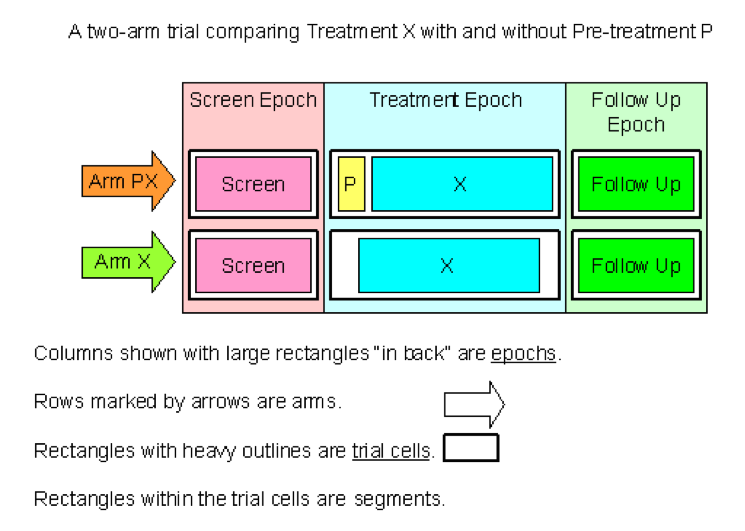
\includegraphics[height=0.35\textheight,clip=true,trim=0 0.5cm 0 0]{./CDISCTrialStructure}%
\caption{Overview of the Trial Structure used in the CDISC Study
  Design Model.}
\label{fig:cdiscstruct}
\end{figure}


To get an idea how this works in practise, the following example shows
a simple clinical trial describing a steady state model, with one
study arm.

\begin{xmlcode}
    <TrialDesign xmlns="http://www.pharmml.org/2013/03/TrialDesign">
        <Structure>
            <!-- Define the trial structure -->
            <Epoch oid="e1">
                <Order>1</Order>
            </Epoch>
            <Arm oid="a1"/>
            <Cell oid="c1">
                <EpochRef oid="e1"/>
                <ArmRef oid="a1"/>
                <SegmentRef oid="s1"/>
            </Cell>
            <Segment oid="s1">
                <ActivityRef oid="a1"/>
            </Segment>
            <Activity oid="a1">
                <Bolus>
                    <DoseAmount>
                        <DoseVar block="main" symbId="D"/>
                        <ct:Assign>
                            <ct:Real>100</ct:Real>
                        </ct:Assign>
                    </DoseAmount>
                    <SteadyState>
                        <EndTime>
                            <ct:SymbRef symbId="tD"/>
                            <ct:Assign><ct:Real>0</ct:Real></ct:Assign>
                        </EndTime>
                        <Interval>
                            <ct:SymbRef block="p1" symbId="tau"/>
                            <ct:Assign><ct:Real>12</ct:Real></ct:Assign>
                        </Interval>
                    </SteadyState>
                </Bolus>
            </Activity>
        </Structure>
        <Population>
            <!-- Define the variability level associated with the
                population -->
            <ct:VariabilityReference>
                <ct:SymbRef blkIdRef="model" symbIdRef="indiv"/>
            </ct:VariabilityReference>
            <!-- Define a template to populate -->
            <IndividualTemplate>
                <IndividualMapping>
                    <ColumnRef xmlns="http://www.pharmml.org/2013/08/Dataset" columnIdRef="id"/>
                </IndividualMapping>
                <ArmMapping>
                    <ColumnRef xmlns="http://www.pharmml.org/2013/08/Dataset" columnIdRef="arm"></ColumnRef>
                </ArmMapping>
                <ReplicateMapping>
                    <ColumnRef xmlns="http://www.pharmml.org/2013/08/Dataset" columnIdRef="rep"/>
                </ReplicateMapping>
            </IndividualTemplate>
            <!-- Populate the tem,plate with data -->
            <DataSet xmlns="http://www.pharmml.org/2013/08/Dataset">
                <Definition>
                    <Column columnId="id" valueType="string" columnNum="1"/>
                    <Column columnId="arm" valueType="string" columnNum="2"/>
                    <Column columnId="rep" valueType="int" columnNum="3"/>
                </Definition>
                <Table>
                    <Row><ct:String>i1</ct:String><ct:String>a1</ct:String><ct:Int>50</ct:Int></Row>
                </Table>
            </DataSet>
        </Population>
    </TrialDesign>
\end{xmlcode}

The CDISC like elements are contained in the \xelem{Structure}
tag and you can see how the study is constructed of a single epoch,
with a single arm and a single cell that contains a single
segment. Note, though that this structure is not hierarchical and the
\xelem{Cell} element joins together the arms, epoch and segments
together. Note that a Cell can span several arms contains several
segments. Finally the segment points to an activity the describes
the steady state dosing regimen. The dosing regimen is very similar
to that used in version 0.1 of \pharmml. The details should be ignored
here and please refer to proposed changes to the dosing regimen in the
section below.

Following on from the \xelem{Structure} element is
\xelem{Population}. This is where we describe the individuals in the
study, their attributes (such as weight, gender etc) and assign them
to an arm of the study. \watchout We define the possible attributes of all
individuals using the \xelem{IndividualTemplate} and then map each
individual to this template using a \xelem{Dataset}. In this simple
example we only have one arm and so we assign all the individuals in
the study to that arm. As a shorthand we provide one individual
definition and state that there are 50 individuals with identical
attributes to this one.

This is obviously useful when simulating a model when (as in this
example) covariates such as weight are calculated for each
individual. An identifier for each individual is created on the fly by
suffixing a sequential number after the identifier. In this case they
would be i1, i2 \ldots i49, i50. While not useful at the moment, such
identifiers will be generated when writing out output to a file. The
\xelem{ReplicateMapping} element is optional and later examples will
explicitly define
 the properties of each individual in the population without
using it.

In this simple example the same amount of dose was administered for
each individual. However, in many models the size of the dose varies
per individual. In the example below you can see more complex trial
design with multiple arms and dosing specified per individual. This
corresponds the trial design describing example 6 in the \pharmml
specification. I've reproduced the figure describing it below (figure
\ref{fig:eg6-trial-design}).

\begin{figure}[htb]
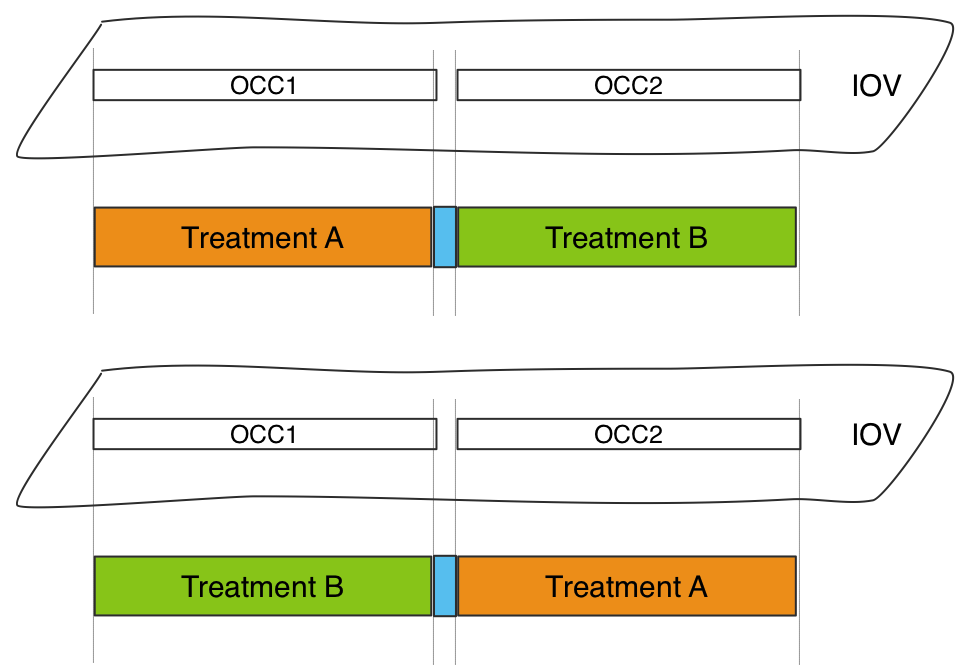
\includegraphics[width=\linewidth]{../pics/iov1simulation_grafio}
\caption{Overview of the trial design used in example 6 of the spec.}
\label{fig:eg6-trial-design}
\end{figure}

\begin{xmlcode}
    <TrialDesign xmlns="http://www.pharmml.org/2013/03/TrialDesign">
        <Structure>
            <Epoch oid="ep1">
                <Order>1</Order>
            </Epoch>
            <Epoch oid="ep2">
                <Order>2</Order>
            </Epoch>
            <Epoch oid="ep3">
                <Order>3</Order>
            </Epoch>
            <Arm oid="a1"/>
            <Arm oid="a2"/>
            <Cell oid="c1">
                <EpochRef oid="e1" />
                <ArmRef oid="a1"/>
                <SegmentRef oid="ta"/>
            </Cell>
            <Cell oid="c2">
                <EpochRef oid="e1" />
                <ArmRef oid="a1"/>
                <SegmentRef oid="tb"/>
            </Cell>
            <Cell oid="c3">
                <EpochRef oid="e2" />
                <ArmRef oid="a1"/>
                <ArmRef oid="a2"/>
                <SegmentRef oid="wash"/>
            </Cell>
            <Cell oid="c4">
                <EpochRef oid="e3"/>
                <ArmRef oid="a1"/>
                <SegmentRef oid="tb"/>
            </Cell>
            <Cell oid="c5">
                <EpochRef oid="e3"/>
                <ArmRef oid="a2"/>
                <SegmentRef oid="ta"/>
            </Cell>
            <Segment oid="ta">
                <ActivityRef oid="d1"/>
            </Segment>
            <Segment oid="tb">
                <ActivityRef oid="d2"/>
            </Segment>
            <Segment oid="wash">
                <ActivityRef oid="w1"/>
            </Segment>
            <Activity oid="d1">
                <Bolus>
                <!-- SNIP -->
                </Bolus>
            </Activity>
            <Activity oid="d2">
                <Bolus>
                <!-- SNIP -->
                </Bolus>
            </Activity>
            <Activity oid="w1">
                <Washout/>
            </Activity>
            <ObservationsEvent oid="occasions">
                <ArmRef oid="a1"/>
                <ArmRef oid="a2"/>
                <ct:VariabilityReference>
                    <ct:SymbRef block="model" symbId="iov"></ct:SymbRef>
                </ct:VariabilityReference>
                <ObservationGroup oid="occ1">
                    <EpochRef oid="ep1"/>
                </ObservationGroup>
                <ObservationGroup oid="occ2">
                    <EpochRef oid="ep3"/>
                </ObservationGroup>
            </ObservationsEvent>
        </Structure>
        <Population>
            <ct:VariabilityReference>
                <ct:SymbRef blkIdRef="model" symbIdRef="indiv"/>
            </ct:VariabilityReference>
            <IndividualTemplate>
                <IndividualMapping>
                    <ds:ColumnRef columnIdRef="id"/>
                </IndividualMapping>
                <ArmMapping>
                    <ds:ColumnRef columnIdRef="arm"/>
                </ArmMapping>
                <CovariateMapping>
                    <ds:ColumnRef columnIdRef="sex"></ds:ColumnRef>
                    <ct:SymbRef blkIdRef="c1" symbIdRef="Sex"/>
                </CovariateMapping>
                <IVDependentMapping>
                    <ds:ColumnRef columnIdRef="treat-tab"/>
                    <EpochMapping>
                        <ds:ColumnRef columnIdRef="epoch"/>
                    </EpochMapping>
                    <CovariateMapping>
                        <ds:ColumnRef columnIdRef="treat"></ds:ColumnRef>
                        <ct:SymbRef blkIdRef="c1" symbIdRef="Treat"/>
                    </CovariateMapping>
                </IVDependentMapping>
            </IndividualTemplate>
            <ds:DataSet>
                <ds:Definition>
                    <ds:Column columnId="id" valueType="string" columnNum="1"/>
                    <ds:Column columnId="arm" valueType="string" columnNum="2"/>
                    <ds:Column columnId="sex" valueType="string" columnNum="3"/>
                    <ds:Table tableId="treat-tab">
                        <ds:Column columnId="epoch" valueType="string" columnNum="1"/>
                        <ds:Column columnId="treat" valueType="string" columnNum="2"/>
                    </ds:Table>
                </ds:Definition>
                <ds:Table>
                    <ds:Row>
                        <ct:String>i1</ct:String>
                        <ct:String>a1</ct:String>
                        <ct:String>M</ct:String>
                        <ds:Table>
                            <ds:Row><ct:String>ep1</ct:String><ct:String>A</ct:String></ds:Row>
                            <ds:Row><ct:String>ep3</ct:String><ct:String>B</ct:String></ds:Row>
                        </ds:Table>
                    </ds:Row>
                    <ds:Row>
                        <ct:String>i2</ct:String>
                        <ct:String>a1</ct:String>
                        <ct:String>M</ct:String>
                        <ds:Table>
                            <ds:Row><ct:String>ep1</ct:String><ct:String>A</ct:String></ds:Row>
                            <ds:Row><ct:String>ep3</ct:String><ct:String>B</ct:String></ds:Row>
                        </ds:Table>
                    </ds:Row>
                    <!-- Snip -->
                    <ds:Row>
                        <ct:String>i8</ct:String>
                        <ct:String>a2</ct:String>
                        <ct:String>F</ct:String>
                        <ds:Table>
                            <ds:Row><ct:String>ep1</ct:String><ct:String>B</ct:String></ds:Row>
                            <ds:Row><ct:String>ep3</ct:String><ct:String>A</ct:String></ds:Row>
                        </ds:Table>
                    </ds:Row>
                    <!-- Snip -->
                    <ds:Row>
                        <ct:String>i10</ct:String>
                        <ct:String>a2</ct:String>
                        <ct:String>M</ct:String>
                        <ds:Table>
                            <ds:Row><ct:String>ep1</ct:String><ct:String>B</ct:String></ds:Row>
                            <ds:Row><ct:String>ep3</ct:String><ct:String>A</ct:String></ds:Row>
                        </ds:Table>
                    </ds:Row>
                </ds:Table>
            </ds:DataSet>
        </Population>
    </TrialDesign>
\end{xmlcode}

In the above example you can see that the more complex trial design
structure is encoded, hopefully as you would expect. Note that the
washout is now defined clearly as an epoch. The new feature that was
not shown in the previous example is the definition of the
occasion as an ObservationsEvent. As you can see this enables us to
define a set of observations, and map them to a variability level. The
duration of each observation (specified by the
\xelem{ObservationGroup} element) can be defined as the duration of a
specified epoch (as in this example) or can be a time period. The
later only makes sense if the epochs define time periods
too\footnote{Note that if each epoch specifies a time period then an
  ObservationEvent can specify a time period that spans multiple
  epochs.}. The \xelem{ObservationsEvent} is associated with an arm,
which means that different sets of inter-occasion variability can be
applied to different arms. I'm not sure if this makes sense or whether
the \xelem{ObservationsEvent} should apply to all arm at the same time
--- and therefore all subjects in the study.

Note also that the definition of the population is richer, with
covariates being defined for each individual. In this example too each
individual in the study is being explicitly defined. Take particular
note of the \xelem{IVDependentMapping} element, which is a child of
the \xelem{IndividualTemplate} element. This is how we define
covariates that are dependent on the independent variable (typically
time). In this example we specify a value for the covariate to be used
during a given epoch\footnote{It is also possible to specify a
  time-point which specifies from which time in the study the
  covariate value applies}. \watchout As you can see this requires the dataset
to be richer since each time-dependent covariate value effectively
defines a table of information ro each row in the dataset. This is
explained in more detail in section (\ref{sec:dataset-refactoring}).

Perhaps the most complex example is from the Chan and Holford
model\footnote{ref} that defines the most complex trial design
structure that we have so far encoded. It was only possible to encode
this using the data-file approach in the previous version of \pharmml
and even then we had to fix a problem where this method could not
define steady state dosing. As it stands this model cannot be encoded
in version 0.1 of \pharmml. The example is below:

\begin{xmlcode}
    <TrialDesign xmlns="http://www.pharmml.org/2013/03/TrialDesign">
        <Structure>
            <Epoch oid="m1">
                <Start>
                    <ct:Real>0</ct:Real>
                </Start>
                <End>
                    <ct:Real>90</ct:Real>
                </End>
                <Order>1</Order>
            </Epoch>
            <Epoch oid="m6">
                <Start>
                    <ct:Real>408</ct:Real>
                </Start>
                <End>
                    <ct:Real>499</ct:Real>
                </End>
                <Order>2</Order>
            </Epoch>
            <Epoch oid="m12">
                <Start>
                    <ct:Real>908</ct:Real>
                </Start>
                <End>
                    <ct:Real>9999</ct:Real>
                </End>
                <Order>3</Order>
            </Epoch>
            <Epoch oid="m24">
                <Start>
                    <ct:Real>1908</ct:Real>
                </Start>
                <End>
                    <ct:Real>1999</ct:Real>
                </End>
                <Order>4</Order>
            </Epoch>
            <Epoch oid="m48">
                <Start>
                    <ct:Real>3908</ct:Real>
                </Start>
                <End>
                    <ct:Real>3999</ct:Real>
                </End>
                <Order>5</Order>
            </Epoch>
            <Arm oid="a1"/>
            <Cell oid="c1">
                <EpochRef oidRef="m1"/>
                <ArmRef oidRef="a1"/>
                <SegmentRef oidRef="s1"/>
            </Cell>
            <Cell oid="c2">
                <EpochRef oidRef="m6"/>
                <ArmRef oidRef="a1"/>
                <SegmentRef oidRef="s2"/>
            </Cell>
            <Cell oid="c4">
                <EpochRef oidRef="m12"/>
                <ArmRef oidRef="a1"/>
                <SegmentRef oidRef="s2"/>
            </Cell>
            <Cell oid="c5">
                <EpochRef oidRef="m24"/>
                <ArmRef oidRef="a1"/>
                <SegmentRef oidRef="s2"/>
            </Cell>
            <Cell oid="c6">
                <EpochRef oidRef="m48"/>
                <ArmRef oidRef="a1"/>
                <SegmentRef oidRef="s2"/>
            </Cell>
            <Segment oid="s1">
                <ActivityRef oidRef="exoinf"/>
            </Segment>
            <Segment oid="s2">
                <ActivityRef oidRef="exoinf"/>
                <ActivityRef oidRef="oralss"/>
            </Segment>
            <Activity oid="exoinf">
                <Infusion>
                    <DoseAmount inputType="target">
                        <ct:SymbRef blkIdRef="sm1" symbIdRef="Ac"></ct:SymbRef>
                    </DoseAmount>
                    <Duration>
                        <ct:SymbRef blkIdRef="pm1" symbIdRef="TTK0"/>
                    </Duration>
                </Infusion>
            </Activity>
            <Activity oid="oralss">
                <Infusion>
                    <DoseAmount inputType="target">
                        <ct:SymbRef blkIdRef="sm1" symbIdRef="Ac"></ct:SymbRef>
                        <ct:Assign><ct:SymbRef blkIdRef="pm1" symbIdRef="Css"/></ct:Assign>
                    </DoseAmount>
                    <SteadyState>
                        <EndTime>
                            <ct:Assign>
                                <ct:Real>0</ct:Real>
                            </ct:Assign>
                        </EndTime>
                    </SteadyState>
                    <Rate><ct:SymbRef blkIdRef="sm1" symbIdRef="R1"></ct:SymbRef></Rate>
                </Infusion>
            </Activity>
            <ObservationsEvent oid="occ">
                <ArmRef oidRef="a1"/>
                <ct:Name>Occasions</ct:Name>
                <ct:VariabilityReference>
                    <ct:SymbRef symbIdRef="occ"/>
                </ct:VariabilityReference>
                <ObservationGroup oid="occ1">
                   <Period> <Start>
                        <ct:Real>0</ct:Real>
                    </Start>
                    <End>
                        <ct:Real>24</ct:Real>
                    </End></Period>
                </ObservationGroup>
                <ObservationGroup oid="occ2">
                    <Period><Start>
                        <ct:Real>72</ct:Real>
                    </Start>
                    <End>
                        <ct:Real>90</ct:Real>
                    </End></Period>
                </ObservationGroup>
                <ObservationGroup oid="occ3">
                    <Period><Start>
                        <ct:Real>408</ct:Real>
                    </Start>
                    <End>
                        <ct:Real>457</ct:Real>
                    </End></Period>
                </ObservationGroup>
                <ObservationGroup oid="occ4">
                    <Period><Start>
                        <ct:Real>481</ct:Real>
                    </Start>
                    <End>
                        <ct:Real>499</ct:Real>
                    </End></Period>
                </ObservationGroup>
                <ObservationGroup oid="occ5">
                   <Period> <Start>
                        <ct:Real>908</ct:Real>
                    </Start>
                    <End>
                        <ct:Real>957</ct:Real>
                    </End></Period>
                </ObservationGroup>
                <ObservationGroup oid="occ6">
                    <Period><Start>
                        <ct:Real>981</ct:Real>
                    </Start>
                    <End>
                        <ct:Real>999</ct:Real>
                    </End></Period>
                </ObservationGroup>
                <ObservationGroup oid="occ7">
                    <Period><Start>
                        <ct:Real>1908</ct:Real>
                    </Start>
                    <End>
                        <ct:Real>1957</ct:Real>
                    </End></Period>
                </ObservationGroup>
                <ObservationGroup oid="occ8">
                   <Period> <Start>
                        <ct:Real>1981</ct:Real>
                    </Start>
                    <End>
                        <ct:Real>1999</ct:Real>
                    </End></Period>
                </ObservationGroup>
                <ObservationGroup oid="occ9">
                    <Period><Start>
                        <ct:Real>3908</ct:Real>
                    </Start>
                    <End>
                        <ct:Real>3957</ct:Real>
                    </End></Period>
                </ObservationGroup>
                <ObservationGroup oid="occ10">
                    <Period><Start>
                        <ct:Real>3981</ct:Real>
                    </Start>
                    <End>
                        <ct:Real>3999</ct:Real>
                    </End></Period>
                </ObservationGroup>
            </ObservationsEvent>
            <ObservationsEvent oid="trial">
                <ArmRef oidRef="a1"/>
                <ct:Name>Trials</ct:Name>
                <ct:VariabilityReference>
                    <ct:SymbRef symbIdRef="occ"/>
                </ct:VariabilityReference>
                <ObservationGroup oid="t1">
                    <EpochRef oidRef="m1"/>
                </ObservationGroup>
                <ObservationGroup oid="t1">
                    <EpochRef oidRef="m6"/>
                </ObservationGroup>
                <ObservationGroup oid="t1">
                    <EpochRef oidRef="m12"/>
                </ObservationGroup>
                <ObservationGroup oid="t4">
                    <EpochRef oidRef="m24"/>
                </ObservationGroup>
                <ObservationGroup oid="t5">
                    <EpochRef oidRef="m48"/>
                </ObservationGroup>
            </ObservationsEvent>
        </Structure>
        <Population>
            <ct:VariabilityReference>
                <ct:SymbRef blkIdRef="model" symbIdRef="indiv"/>
            </ct:VariabilityReference>
            <IndividualTemplate>
                <IndividualMapping>
                    <ds:ColumnRef columnIdRef="id"/>
                </IndividualMapping>
                <ArmMapping>
                    <ds:ColumnRef columnIdRef="arm"/>
                </ArmMapping>
                <IVDependentMapping>
                    <ds:ColumnRef columnIdRef="td-weight"/>
                    <EpochMapping>
                        <ds:ColumnRef columnIdRef="epoch"/>
                    </EpochMapping>
                    <CovariateMapping>
                        <ds:ColumnRef columnIdRef="wt"></ds:ColumnRef>
                        <ct:SymbRef blkIdRef="cm1" symbIdRef="W"/>
                    </CovariateMapping>
                </IVDependentMapping>
            </IndividualTemplate>
            <ds:DataSet>
                <ds:Definition>
                    <ds:Column columnId="id" valueType="string" columnNum="1"/>
                    <ds:Column columnId="arm" valueType="string" columnNum="2"/>
                    <ds:Table>
                        <ds:Column columnId="epoch" valueType="string" columnNum="1"/>
                        <ds:Column columnId="wt" valueType="real" columnNum="2"/>
                    </ds:Table>
                </ds:Definition>
                <ds:Table>
                    <ds:Row>
                        <ct:String>i552</ct:String><ct:String>a1</ct:String>
                            <ds:Table>
                                <ds:Row><ct:String>m1</ct:String><ct:Real>73</ct:Real></ds:Row>
                                <ds:Row><ct:String>m6</ct:String><ct:Real>70</ct:Real></ds:Row>
                                <ds:Row><ct:String>m12</ct:String><ct:Real>73</ct:Real></ds:Row>
                                <ds:Row><ct:String>m24</ct:String><ct:Real>71</ct:Real></ds:Row>
                                <ds:Row><ct:String>m48</ct:String><ct:Real>69</ct:Real></ds:Row>
                            </ds:Table>
                    </ds:Row>
                    <ds:Row>
                        <ct:String>i553</ct:String><ct:String>a1</ct:String>
                        <ds:Table>
                            <ds:Row><ct:String>m1</ct:String><ct:Real>75</ct:Real></ds:Row>
                            <ds:Row><ct:String>m6</ct:String><ct:Real>74</ct:Real></ds:Row>
                            <ds:Row><ct:String>m12</ct:String><ct:Real>75</ct:Real></ds:Row>
                            <ds:Row><ct:String>m24</ct:String><ct:Real>72</ct:Real></ds:Row>
                            <ds:Row><ct:String>m48</ct:String><ct:Real>70</ct:Real></ds:Row>
                        </ds:Table>
                    </ds:Row>
                </ds:Table>
            </ds:DataSet>
        </Population>
        <IndividualDosing>
                <ActivityRef oidRef="exoinf"/>
                <IndividualRef columnIdRef="id"/>
                <DoseAmount columnIdRef="dose"/>
                <DosingTime columnIdRef="t"/>
                <DataSet xmlns="http://www.pharmml.org/2013/08/Dataset">
                    <Definition>
                        <Column columnNum="1" columnId="id" valueType="string"/>
                        <Column columnNum="2" columnId="t" valueType="real"/>
                        <Column columnNum="3" columnId="dose" valueType="real"/>
                    </Definition>
                    <Table>
                        <ds:Row xmlns="http://www.pharmml.org/2013/03/CommonTypes">
                            <String>i552</String><Real>0</Real><Real>740.37</Real>
                            <String>i552</String><Real>72</Real><Real>740.37</Real>
                            <String>i552</String><Real>409</Real><Real>709.94</Real>
                            <String>i552</String><Real>481</Real><Real>709.94</Real>
                            <String>i552</String><Real>909</Real><Real>740.94</Real>
                            <String>i552</String><Real>981</Real><Real>740.94</Real>
                            <String>i552</String><Real>1909</Real><Real>720.08</Real>
                            <String>i552</String><Real>1981</Real><Real>720.08</Real>
                            <String>i552</String><Real>3909</Real><Real>699.8</Real>
                            <String>i552</String><Real>3981</Real><Real>699.8</Real>
                        </ds:Row>
                    </Table>
                </DataSet>
        </IndividualDosing>
    </TrialDesign>
\end{xmlcode}

This uses all the components that you have seen in the previous
examples, with the addition of the \xelem{IndividualDosing}
element. Its purpose is to provide per individual dosing information
for a given dosing activity (specified by
\verb|<ActivityRef oidRef="inf1"/>|).  Note that in this example the
dose varies with time, but of course it need not do, in which case the
time column and \xelem{DosingTime} record are omitted. Note that the
type of each value is specified explicitly so it is clear whether the
value is compatible with the information it is being mapped to. If we
need dosing information for more than one dosing activity then
multiple \xelem{IndividualDosing} sections can be defined.

\subsubsection{Higher levels of variability}

\watchout The redesigned trial design can handle levels of variability above the
level of individual variability. We can do this by assigning
additional attributes to the definition of an individual, that are not
covariates, called \emph{Demographic Attributes}\footnote{Note that
  this is what I call my working name. There may be a better one we
  should use instead.}. There will not doubt be a better name for
this. As usual this is best understood with an example. First the
variability model we are using looks like this:
%
\begin{xmlcode}
<VariabilityModel id="e1" blkId="model">
    <Level symbId="country">
        <ct:Name>Country</ct:Name>
    </Level>
    <Level symbId="centre">
        <ct:Name>Study Centre</ct:Name>
        <ParentLevel>
            <ct:SymbRef symbIdRef="country"/>
        </ParentLevel>
    </Level>
    <Level symbId="indiv">
        <ct:Name>Individual Variability</ct:Name>
        <ParentLevel>
            <ct:SymbRef symbIdRef="centre"/>
        </ParentLevel>
    </Level>
</VariabilityModel>
<VariabilityModel blkId="obsErr">
    <Level symbId="residual">
        <ct:Name>Residual Error</ct:Name>
        <ParentLevel>
            <ct:SymbRef blkIdRef="model" symbIdRef="indiv"/>
        </ParentLevel>
    </Level>
</VariabilityModel>
\end{xmlcode}
%
As you can see there is a country and centre hierarchy above an
individual. In PharmML we therefore assign each individual to a
country and a centre and link these attributes to the appropriate
variability level. These variability levels are then used in the model
definition in the usual way:
%
\begin{xmlcode}
<!-- kout -->
<SimpleParameter symbId="pop_kout"/>
<SimpleParameter symbId="omega_kout"/>
<RandomVariable symbId="eta_kout">
  <!-- Snip -->
</RandomVariable>
<SimpleParameter symbId="gamma1_kout"/>
<RandomVariable symbId="kappa1_kout">
    <ct:VariabilityReference>
        <ct:SymbRef symbIdRef="centre"/>
    </ct:VariabilityReference>
    <NormalDistribution xmlns="http://www.uncertml.org/3.0" definition="http://www.uncertml.org/NormalDistribution">
        <mean><rVal>0</rVal></mean>
        <stddev><var varId="gamma1_kout"/></stddev>
    </NormalDistribution>
</RandomVariable>
<SimpleParameter symbId="gamma2_kout"/>
<RandomVariable symbId="kappa2_kout">
    <ct:VariabilityReference>
        <ct:SymbRef symbIdRef="country"/>
    </ct:VariabilityReference>
    <NormalDistribution xmlns="http://www.uncertml.org/3.0" definition="http://www.uncertml.org/NormalDistribution">
        <mean><rVal>0</rVal></mean>
        <stddev><var varId="gamma2_kout"/></stddev>
    </NormalDistribution>
</RandomVariable>
<IndividualParameter symbId="kout">
    <GaussianModel>
        <Transformation>log</Transformation>
        <LinearCovariate>
            <PopulationParameter>
                <ct:Assign>
                    <ct:SymbRef symbIdRef="pop_kout"></ct:SymbRef>
                </ct:Assign>
            </PopulationParameter>
        </LinearCovariate>
        <RandomEffects>
            <ct:SymbRef symbIdRef="eta_kout"/>
            <ct:SymbRef symbIdRef="kappa1_kout"/>
            <ct:SymbRef symbIdRef="kappa2_kout"/>
        </RandomEffects>
    </GaussianModel>
</IndividualParameter>
\end{xmlcode}

The first step is to define the possible values for each attribute and
then map them to the variability level. The example below shows a
definition of the demographic attribute \texttt{country}. Its possible
values are given as `UK' and `USA', which means
individuals can only be assigned these values. It is also associated
with the variability level also called \texttt{country} in the
variability model. This indicates that there is random variability
between individuals from different countries.
%
\begin{xmlcode}
<Demographic oid="country">
    <ct:VariabilityReference>
        <ct:SymbRef blkIdRef="model" symbIdRef="country"/>
    </ct:VariabilityReference>
    <ct:String>UK</ct:String>
    <ct:String>US</ct:String>
</Demographic>
\end{xmlcode}

Now that we have defined a demographic attribute it can be mapped in
the \xelem{IndividualTemplate} as you would a covariate and then the
country and centre of each individual defined in the dataset. The
complete example is shown below:
%
\begin{xmlcode}
        <Population>
            <ct:VariabilityReference>
                <ct:SymbRef blkIdRef="model" symbIdRef="indiv"/>
            </ct:VariabilityReference>
            <Demographic oid="country">
                <ct:VariabilityReference>
                    <ct:SymbRef blkIdRef="model" symbIdRef="country"/>
                </ct:VariabilityReference>
                <ct:String>UK</ct:String>
                <ct:String>US</ct:String>
            </Demographic>
            <Demographic oid="centre">
                <ct:VariabilityReference>
                    <ct:SymbRef blkIdRef="model" symbIdRef="centre"/>
                </ct:VariabilityReference>
                <ct:String>centre1</ct:String>
                <ct:String>centre2</ct:String>
            </Demographic>
            <IndividualTemplate>
                <IndividualMapping><!-- Need to add rule about what is the key of the dataset -->
                    <ds:ColumnRef  columnIdRef="id"/>
                </IndividualMapping>
                <ArmMapping>
                    <ds:ColumnRef  columnIdRef="arm"/>
                </ArmMapping>
                <DemographicMapping>
                    <ds:ColumnRef  columnIdRef="cty"></ds:ColumnRef >
                    <ct:OidRef oidRef="country"/>
                </DemographicMapping>
                <DemographicMapping>
                    <ds:ColumnRef  columnIdRef="ctr"></ds:ColumnRef >
                    <ct:OidRef oidRef="centre"/>
                </DemographicMapping>
                <ReplicateMapping>
                    <ds:ColumnRef  columnIdRef="reps"/>
                </ReplicateMapping>
            </IndividualTemplate>
            <ds:DataSet>
            <ds:Definition>
                <ds:Column columnId="id" valueType="string" columnNum="1"/>
                <ds:Column columnId="arm" valueType="string" columnNum="2"/>
                <ds:Column columnId="cty" valueType="string" columnNum="3"/>
                <ds:Column columnId="ctr" valueType="string" columnNum="4"/>
                <ds:Column columnId="reps" valueType="int" columnNum="5"/>
            </ds:Definition>
                <ds:Table>
                    <ds:Row>
                        <ct:String>i1</ct:String><ct:String>a1</ct:String><ct:String>UK</ct:String><ct:String>centre1</ct:String><ct:Int>20</ct:Int>
                    </ds:Row>
                    <ds:Row>
                        <ct:String>i2</ct:String><ct:String>a2</ct:String><ct:String>UK</ct:String><ct:String>centre2</ct:String><ct:Int>20</ct:Int>
                    </ds:Row>
                    <ds:Row>
                        <ct:String>i3</ct:String><ct:String>a3</ct:String><ct:String>US</ct:String><ct:String>centre1</ct:String><ct:Int>20</ct:Int>
                    </ds:Row>
                    <ds:Row>
                        <ct:String>i4</ct:String><ct:String>a4</ct:String><ct:String>US</ct:String><ct:String>centre2</ct:String><ct:Int>20</ct:Int>
                    </ds:Row>
                    <!-- Snip -->
                </ds:Table>
            </ds:DataSet>            
        </Population>
\end{xmlcode}

\subsection{Simplifying the Estimation Step}

A by-product of the redesign of the Trial Design structure is that the
estimation and simulation steps can be considerably
simplified. Perhaps the greatest simplification is with the
\xelem{SimulationStep} which can drop the need to specify the design
in a data file. It now just needs to define initial values and specify
what observations to simulate. A by-product of the re-design is that
we also fix one of the unresolved issues in version 0.1 of
\pharmml. It wasn't clear how to simulate only one epoch since it was
possible for each epoch to have the same time period when separated by
a washout. Now however the epochs must specify consecutive time
periods so the simulation can easily be defined to span all the time
periods in all the epochs of the study.

Finally the use of a data-file in the estimation step becomes very
simple. See for example the estimation step of the Holford and Chan
model:
%
\begin{xmlcode}
<EstimationStep oid="estTask1">
    <ObjectiveDataSet>
        <IndividualMapping>
            <ds:ColumnRef  columnIdRef="id"/>
        </IndividualMapping>
        <VariableMapping>
            <ds:ColumnRef  columnIdRef="time"/>
            <ct:SymbRef symbIdRef="t"/>
            <Interpolation>
                <Method name="default"/>
            </Interpolation>
        </VariableMapping>
        <VariableMapping>
            <ds:ColumnRef  columnIdRef="DV"/>
            <ct:SymbRef blkIdRef="om1" symbIdRef="CP"></ct:SymbRef>
            <Interpolation>
                <Method name="default"/>
            </Interpolation>
        </VariableMapping>
        <ds:DataSet>
            <ds:Definition>
                <ds:Column columnNum="1" columnId="id" valueType="string"/>
                <ds:Column columnNum="2" columnId="time" valueType="real"/>
                <ds:Column columnNum="3" columnId="DV" valueType="real"/>
            </ds:Definition>
            <ds:Table>
                <ds:Row>
                    <ct:String>i552</ct:String><ct:Real>0</ct:Real><ct:Real>0</ct:Real>
                </ds:Row>
                <ds:Row>
                    <ct:String>i552</ct:String><ct:Real>1</ct:Real><ct:Real>6.11</ct:Real>
                </ds:Row>
                <ds:Row>
                    <ct:String>i552</ct:String><ct:Real>1.5</ct:Real><ct:Real>7.38</ct:Real>
                </ds:Row>
                <ds:Row>
                    <ct:String>i552</ct:String><ct:Real>2</ct:Real><ct:Real>7.73</ct:Real>
                </ds:Row>
                <!-- Snip -->
            </ds:Table>
        </ds:DataSet>
    </ObjectiveDataSet>
    <ParametersToEstimate>
      <!-- Snip -->
    </ParametersToEstimate>
    <Operation order="1" opType="estPop">
        <Algorithm definition="FOCEI"></Algorithm>
    </Operation>
</EstimationStep>
\end{xmlcode}
%
Here the mapping of the objective data to the model becomes trivial and
this simplicity enables us to focus on issues we neglected when the
\xelem{EstimationStep} was more complicated. You will notice that each
\xelem{VariableMapping} element contains an \xelem{Interpolation}
element. This allows us to specify how the data should be interpolated
during the estimation procedure. The only available method at the
moment is \emph{default} so clearly this needs more work, but the
objective is clear.

\watchout We can extend this approach to also support multiple datasets within
one estimation step. Why? Well possible scenarios are:
\begin{enumerate}
\item You have separate PK and PD measurements taken at different
  time-points.
\item You have replicate observations (possible obtained using
  different assays or instruments) and you want to map each replicate
  to a different error model.
\end{enumerate}
The hypothetical example below shows, how you might describe the first
case:
\begin{xmlcode}
<EstimationStep oid="estTask1">
    <ObjectiveDataSet>
        <IndividualMapping>
            <ds:ColumnRef  columnIdRef="id"/>
        </IndividualMapping>
        <VariableMapping>
            <ds:ColumnRef  columnIdRef="time"/>
            <ct:SymbRef symbIdRef="t"/>
            <Interpolation>
                <Method name="default"/>
            </Interpolation>
        </VariableMapping>
        <VariableMapping>
            <ds:ColumnRef  columnIdRef="DV"/>
            <ct:SymbRef blkIdRef="om1" symbIdRef="CP"></ct:SymbRef>
            <Interpolation>
                <Method name="default"/>
            </Interpolation>
        </VariableMapping>
        <ds:DataSet>
            <ds:Definition>
                <ds:Column columnNum="1" columnId="id" valueType="string"/>
                <ds:Column columnNum="2" columnId="time" valueType="real"/>
                <ds:Column columnNum="3" columnId="DV" valueType="real"/>
            </ds:Definition>
            <ds:Table>
                <ds:Row>
                    <ct:String>i552</ct:String><ct:Real>0</ct:Real><ct:Real>0</ct:Real>
                </ds:Row>
                <ds:Row>
                    <ct:String>i552</ct:String><ct:Real>1</ct:Real><ct:Real>5</ct:Real>
                </ds:Row>
                <ds:Row>
                    <ct:String>i552</ct:String><ct:Real>4</ct:Real><ct:Real>9</ct:Real>
                </ds:Row>
                <ds:Row>
                    <ct:String>i552</ct:String><ct:Real>6</ct:Real><ct:Real>11</ct:Real>
                </ds:Row>
                <!-- Snip -->
            </ds:Table>
        </ds:DataSet>
    </ObjectiveDataSet>
    <ObjectiveDataSet>
        <IndividualMapping>
            <ds:ColumnRef  columnIdRef="id"/>
        </IndividualMapping>
        <VariableMapping>
            <ds:ColumnRef  columnIdRef="time"/>
            <ct:SymbRef symbIdRef="t"/>
            <Interpolation>
                <Method name="default"/>
            </Interpolation>
        </VariableMapping>
        <VariableMapping>
            <ds:ColumnRef  columnIdRef="DV"/>
            <ct:SymbRef blkIdRef="om1" symbIdRef="CP"></ct:SymbRef>
            <Interpolation>
                <Method name="default"/>
            </Interpolation>
        </VariableMapping>
        <ds:DataSet>
            <ds:Definition>
                <ds:Column columnNum="1" columnId="id" valueType="string"/>
                <ds:Column columnNum="2" columnId="time" valueType="real"/>
                <ds:Column columnNum="3" columnId="DV" valueType="real"/>
            </ds:Definition>
            <ds:Table>
                <ds:Row>
                    <ct:String>i552</ct:String><ct:Real>0</ct:Real><ct:Real>0</ct:Real>
                </ds:Row>
                <ds:Row>
                    <ct:String>i552</ct:String><ct:Real>6</ct:Real><ct:Real>0</ct:Real>
                </ds:Row>
                <ds:Row>
                    <ct:String>i552</ct:String><ct:Real>12</ct:Real><ct:Real>10</ct:Real>
                </ds:Row>
                <ds:Row>
                    <ct:String>i552</ct:String><ct:Real>24</ct:Real><ct:Real>20</ct:Real>
                </ds:Row>
                <ds:Row>
                    <ct:String>i552</ct:String><ct:Real>36</ct:Real><ct:Real>0</ct:Real>
                </ds:Row>
                <ds:Row>
                    <ct:String>i552</ct:String><ct:Real>48</ct:Real><ct:Real>80</ct:Real>
                </ds:Row>
                <!-- Snip -->
            </ds:Table>
        </ds:DataSet>
    </ObjectiveDataSet>
    <ParametersToEstimate>
      <!-- Snip -->
    </ParametersToEstimate>
    <Operation order="1" opType="estPop">
        <Algorithm definition="FOCEI"></Algorithm>
    </Operation>
</EstimationStep>
\end{xmlcode}
%
Here as you can see there are two datasets. The first provides
measurements for the PK variable $\mathrm{Cc}$ and the second for the
effect variable $E$. The example below shows the second case where the
first dataset describes the first set of replicates and the second
dataset the other. Note that we indicate to the observation model
which replicate set it is being assigning a value to an indicator variable.
%
\begin{xmlcode}
<EstimationStep id="estTask1">
    <ObjectiveDataSet>
        <IndividualMapping>
            <ColumnRef oid="id"/>
        </IndividualMapping>
        <ct:VariableAssignment>
            <ct:SymbRef symbId="replicateFlag"/>
            <ct:Assign>
                <ct:Int>1</ct:Int>
            </ct:Assign>
        </ct:VariableAssignment>
        <VariableMapping>
            <ColumnRef oid="time"/>
            <ct:SymbRef symbId="t"/>
            <Interpolation>
                <Method name="default"/>
            </Interpolation>
        </VariableMapping>
        <VariableMapping>
            <ColumnRef oid="DV"/>
            <ct:SymbRef block="om1" symbId="Cc"></ct:SymbRef>
            <Interpolation>
                <Method name="default"/>
            </Interpolation>
        </VariableMapping>
        <ds:DataSet>
            <!-- Snip -->
        </ds:DataSet>
    </ObjectiveDataSet>
    <ObjectiveDataSet>
        <IndividualMapping>
            <ColumnRef oid="id"/>
        </IndividualMapping>
        <ct:VariableAssignment>
            <ct:SymbRef symbId="replicateFlag"/>
            <ct:Assign>
                <ct:Int>2</ct:Int>
            </ct:Assign>
        </ct:VariableAssignment>
        <VariableMapping>
            <ColumnRef oid="time"/>
            <ct:SymbRef symbId="t"/>
            <Interpolation>
                <Method name="default"/>
            </Interpolation>
        </VariableMapping>
        <VariableMapping>
            <ColumnRef oid="DV"/>
            <ct:SymbRef block="om1" symbId="Cc"></ct:SymbRef>
            <Interpolation>
                <Method name="default"/>
            </Interpolation>
        </VariableMapping>
        <ds:DataSet>
            <!-- Snip -->
        </ds:DataSet>
    </ObjectiveDataSet>
    <ParametersToEstimate>
      <!-- Snip -->
    </ParametersToEstimate>
    <EstimationOperation opType="estPop"/>
</EstimationStep>
\end{xmlcode}
% 
Because we can duplicate datasets in this way this allows us to add a
constraint on the datasets we can use. Namely that we only allow one 
row per combination of individual and time. In doing so we can
then permit observations to be defined in an order independent
way. So:
%
\begin{xmlcode}
<ds:Row><ct:String>i552</ct:String><ct:Real>0</ct:Real><ct:Real>0</ct:Real></ds:Row>
<ds:Row><ct:String>i552</ct:String><ct:Real>6</ct:Real><ct:Real>0</ct:Real></ds:Row>
<ds:Row><ct:String>i552</ct:String><ct:Real>12</ct:Real><ct:Real>10</ct:Real></ds:Row>
<ds:Row><ct:String>i552</ct:String><ct:Real>24</ct:Real><ct:Real>20</ct:Real></ds:Row>
<ds:Row><ct:String>i552</ct:String><ct:Real>36</ct:Real><ct:Real>0</ct:Real></ds:Row>
<ds:Row><ct:String>i552</ct:String><ct:Real>48</ct:Real><ct:Real>80</ct:Real></ds:Row>
\end{xmlcode}
%
is therefore equivalent to:
\begin{xmlcode}
<ds:Row><ct:String>i552</ct:String><ct:Real>36</ct:Real><ct:Real>0</ct:Real></ds:Row>
<ds:Row><ct:String>i552</ct:String><ct:Real>0</ct:Real><ct:Real>0</ct:Real></ds:Row>
<ds:Row><ct:String>i552</ct:String><ct:Real>24</ct:Real><ct:Real>20</ct:Real></ds:Row>
<ds:Row><ct:String>i552</ct:String><ct:Real>12</ct:Real><ct:Real>10</ct:Real></ds:Row>
<ds:Row><ct:String>i552</ct:String><ct:Real>6</ct:Real><ct:Real>0</ct:Real></ds:Row>
<ds:Row><ct:String>i552</ct:String><ct:Real>48</ct:Real><ct:Real>80</ct:Real></ds:Row>
\end{xmlcode}
%
Remember that this representation is meant for information exchange
between software tools. For a human reader this may seem more complex
to comprehend, but for software the fact that there are no duplicates
and no order makes the processing and validation of this information
easier.

\subsection{Residual Error Model}

In the last proposal we revised the structure of the residual error
model to remove the assumptions ion the definition - as we did with
the parameter model. Unsurprisingly the criticism of the parameter
model changes in the previous proposal also apply to the residual
error model. Therefore I propose to follow the same approach as above
and have a constrained form and a flexible form. What I call the
\emph{Standard} form is set out in equation 52 in Lavielle \emph{et
  al}. There may be other forms that we wish to include buy at the
moment I encode the \emph{Standard} and the implicit form (the latter
name is consistent with that used for the eponymous parameter model).

\begin{align*}
\intertext{Type 1. (implicit) equation type of residual error model}
y_{ij} &= G(x_{ij}, \psi_{i}, \epsilon_{ij})
\intertext{Type 2. Standard residual error model}
u(y_{ij}) &= u(f(x_{ij},\psi_i)) + g(x_{ij}, \psi_i) \epsilon_{ij},
\quad 1 \leq i \leq N, \quad 1 \leq j \leq n_i
\end{align*}
with:
\begin{itemize}
\item N is the number of subjects,
\item $y_i = (y_{ij}, 1 \leq j \leq n_i)$ are the observations for
  individual $i$, with $n_i$, the number of observations of subject
  $i$,
\item $x_i = (x_{ij}, 1 \leq j \leq n_i)$ are regression variables,
\item $\psi_i$, is the vector of individual parameters of subject i, 
\item $u$ is a function which transforms the model on both sides,
\item $\epsilon_{ij}$ is the residual error,
\item $g$ is a function that defines the standard deviation of the
  residual error.
\end{itemize}

Here the XML is modified to permit the definition of residual error
using both these forms. To illustrate this I will show the following
how a residual error model using a combined model described using both
forms. \watchout Note also that in previous versions multiple residual error
models could be defined per observation model block. This has now been
limited to 1 per model block. This makes the design cleaner and also
means that if more than one residual error is applied then the
parameters associated with each can be conveniently grouped together.

\subsubsection{General Residual Error Model}

In the first from we define the model as follows:
%
\begin{align*}
C_{o_{ij}} &= C_{s_{ij}} + \left(a + b \cdot f(x_{ij}, \psi_{ij}) \right) \epsilon_{C_{ij}}\\
\intertext{where}
a, b & \text{, are parameters,}\\
C_{o} & \text{, is the output of the observations model,}\\
C_{s} & \text{, is the output of the structural model.}
\end{align*}
%
This can be encoded using the implicit definition as follows:
%
\begin{xmlcode}
    <RandomVariable symbId="epsilon_C">
        <VariabilityReference> <!-- This references the variability level -->
            <ct:SymbRef block="obsErr" symbId="residual"/>
        </VariabilityReference>
        <Distribution xmlns="http://www.pharmml.org/2013/03/Uncertainty"
            writtenVersion="0.1">
            <Normal>
              <!-- Snip -->
            </Normal>
        </Distribution>
    </RandomVariable>
    <General  symbId="C">
        <Output>
            <ct:SymbRef block="main" symbId="C"></ct:SymbRef>
        </Output>
        <ct:Assign>
            <!-- C + (combinedErrorModel(a1, b1, C) * epsilon_C) -->
            <math:Equation writtenVersion="0.1">
                <math:Binop op="plus">
                    <math:Var block="main" symbId="C"/> <!-- C_{s} -->
                    <math:Binop op="times">
                        <math:FunctionCall>
                            <math:Var symbId="combinedErrorModel"/>
                            <math:FunctionArgument symbId="a">
                                <math:Var symbId="a1"/>
                            </math:FunctionArgument>
                            <math:FunctionArgument symbId="b">
                                <math:Var symbId="b1"/>
                            </math:FunctionArgument>
                            <math:FunctionArgument symbId="f">
                                <math:Var block="main" symbId="C"/>
                            </math:FunctionArgument>
                        </math:FunctionCall>
                        <math:Var symbId="epsilon_C"/>
                    </math:Binop>
                </math:Binop>
            </math:Equation>
        </ct:Assign>
    </General>
\end{xmlcode}
%
This is very similar to the previous proposal, but I have introduced
the \xelem{General} element to define the type of error model and this
element now defines observation variable, in this case $C$. I will
explain why this was changed later. Note that multiple \xelem{General}
or \xelem{Standard} elements can be defined within a single
\xelem{Continuous} block. This allows multiple observation variables
to be defined within a single \xelem{Continuous} element.  In this
code snippet you can see that the random variable is defined
explicitly and then used in an equation. As with the parameter
proposal above, this provides maximum flexibility and make the
relationship between the random variable, the error model and the
output variable from the structural model. A validation rule we may
wish to apply is that the equation defining the residual error must
contain references to the random variable defined as a child of the
\xelem{Continuous} element.

\subsubsection{Standard Residual Error Model}

Our example standard error model is defined as follows:
%
\begin{align*}
\mathrm{Cc}_{o_{ij}} &= \mathrm{Cc}_{s_{ij}} + g(a_i, b_i, \mathrm{Cc}_{s}) \epsilon_{\mathrm{Cc}_{ij}}\\
\intertext{where}
g(a, b, f) &= a + b f.
\end{align*}
%
This is similar to the structure used in version 0.1 of \pharmml, but
the random variable is defined explicitly, the observation variable is
defined within the \xelem{Standard} element and the output variable,
$\mathrm{Cc_o}$ is defined within the \xelem{Output} element. Also the
error model now does not necessarily need to be defined as a function,
but and be defined as an algebraic equation within the
\xelem{math:Equation} elements (note that in the example below a call
to an equation is used).
%
\begin{xmlcode}
    <RandomVariable symbId="epsilon_Cc">
        <ct:VariabilityReference>
            <ct:SymbRef block="obsErr" symbId="residual"/>
        </ct:VariabilityReference>
        <NormalDistribution xmlns="http://www.uncertml.org/3.0"
            definition="http://www.uncertml.org/distributions/normal">
            <mean><rVal>0</rVal></mean>
            <stddev><var varId="omega_Cc"/></stddev>
        </NormalDistribution>
    </RandomVariable>
    <Standard symbId="Cc">
        <Output>
            <ct:SymbRef block="main" symbId="Cc"></ct:SymbRef>
        </Output>
        <ErrorModel>
            <ct:Assign>
                <math:Equation>
                    <math:FunctionCall>
                        <ct:SymbRef symbId="combinedErrorModel"/>
                        <math:FunctionArgument symbId="a">
                            <ct:SymbRef symbId="a1"/>
                        </math:FunctionArgument>
                        <math:FunctionArgument symbId="b">
                            <ct:SymbRef symbId="b1"/>
                        </math:FunctionArgument>
                        <math:FunctionArgument symbId="f">
                            <math:Equation>
                                <ct:SymbRef block="main" symbId="Cc"/>
                            </math:Equation>
                        </math:FunctionArgument>
                    </math:FunctionCall>
                </math:Equation>
            </ct:Assign>
        </ErrorModel>
        <ResidualError>
            <ct:SymbRef symbId="epsilon_Cc"/>
        </ResidualError>
    </Standard>
\end{xmlcode}

\subsubsection{Correlation}

To correlate residual errors we simply reuse the constructs for
correlation of random variables in the parameter model. This very
simply allows us to implicitly define a covariance or correlation matrix for
the residual errors in the model. Below is a hypothetical example that
illustrates how it works. Note that this example implies that another
observation model, ``o1'', is also defined and the correlation is
between the residual error defined in that model and the one defined here':
%
\begin{xmlcode}
       <ObservationModel blkId="o2">
            <SimpleParameter symbId="a2"/>
            <SimpleParameter symbId="g_C_E"/>
            <RandomVariable symbId="epsilon_E">
                <ct:UnitRef unitId="percent"/>
                <ct:VariabilityReference>
                    <ct:SymbRef blkIdRef="obsErr" symbIdRef="residual"/>
                </ct:VariabilityReference>
                <NormalDistribution xmlns="http://www.uncertml.org/3.0"
                    definition="http://www.uncertml.org/distributions/normal">
                    <mean><rVal>0</rVal></mean>
                    <stddev><var varId="omega_E"/></stddev>
                </NormalDistribution>
            </RandomVariable>
            <Correlation>
                <ct:VariabilityReference>
                    <ct:SymbRef blkIdRef="obsErr" symbIdRef="residual"/>
                </ct:VariabilityReference>
                <RandomVariable1>
                    <ct:SymbRef blkIdRef="o1" symbIdRef="epsilon_C"/>
                </RandomVariable1>
                <RandomVariable2>
                    <ct:SymbRef symbIdRef="epsilon_E"/>
                </RandomVariable2>
                <Covariance>
                    <ct:SymbRef symbIdRef="g_C_E"/>
                </Covariance>
            </Correlation>
            <General symbId="E">
                <ct:UnitRef unitId="percent"/>
                <ct:Assign>
                    <math:Equation>
                        <math:Binop op="plus">
                            <ct:SymbRef blkIdRef="main" symbIdRef="E"/>
                            <math:Binop op="times">
                                <math:FunctionCall>
                                    <ct:SymbRef symbIdRef="constantErrorModel"/>
                                    <math:FunctionArgument symbId="a">
                                        <ct:SymbRef symbIdRef="a2"/>
                                    </math:FunctionArgument>
                                </math:FunctionCall>
                                <ct:SymbRef symbIdRef="epsilon_E"/>
                            </math:Binop>
                        </math:Binop>
                    </math:Equation>
                </ct:Assign>
            </General>
        </ObservationModel>
\end{xmlcode}

\subsubsection{Parameters with random effects}

\watchout In some error models it is desirable to use parameters in the error
model that have random effects. This was not permitted in the previous
revision of this proposal, however, it has been introduced here. An
example of such a model is taken from Maciej's error model document:
%
\begin{align*}
a_i &= a_{\mathit{pop}} \exp(\eta_{a,i,j}); \quad eta_{a,ij} ~ N(0, \omega^2_a)\\
b_i &= b_{\mathit{pop}} \exp(\eta_{b,i,j}); \quad eta_{b,ij} ~ N(0, \omega^2_b)\\
W_{i j} &= \sqrt{a^2_i + b^2_2 f^2_{ij}}\\
y_{ij} &= f_{ij} + W_{ij} \epsilon_{i j}; \quad e_{ij} ~ N(0,1)
\end{align*}
%
In this example we can represent the parameters $a$ and $b$ as
individual parameters in \pharmml as follows:
%
\begin{xmlcode}
        <ObservationModel blkId="example">
            <SimpleParameter symbId="pop_a"/>
            <RandomVariable symbId="eta_a">
                <ct:VariabilityReference>
                    <ct:SymbRef blkIdRef="model" symbIdRef="indiv"/>
                </ct:VariabilityReference>
                <NormalDistribution xmlns="http://www.uncertml.org/3.0" definition="">
                    <mean><rVal>0</rVal></mean>
                    <stddev><var varId="omega_a"/></stddev>
                </NormalDistribution>
            </RandomVariable>
            <IndividualParameter symbId="a">
                <ct:Assign>
                    <math:Equation>
                        <math:Binop op="times">
                            <ct:SymbRef symbIdRef="pop_a"></ct:SymbRef>
                            <math:Uniop op="exp">
                                <ct:SymbRef symbIdRef="eta_a"></ct:SymbRef>
                            </math:Uniop>
                        </math:Binop>
                    </math:Equation>
                </ct:Assign>
            </IndividualParameter>
            <SimpleParameter symbId="pop_b"/>
            <RandomVariable symbId="eta_b">
                <ct:VariabilityReference>
                    <ct:SymbRef blkIdRef="model" symbIdRef="indiv"/>
                </ct:VariabilityReference>
                <NormalDistribution xmlns="http://www.uncertml.org/3.0" definition="">
                    <mean><rVal>0</rVal></mean>
                    <stddev><var varId="omega_b"/></stddev>
                </NormalDistribution>
            </RandomVariable>
            <IndividualParameter symbId="b">
                <ct:Assign>
                    <math:Equation>
                        <math:Binop op="times">
                            <ct:SymbRef symbIdRef="pop_b"></ct:SymbRef>
                            <math:Uniop op="exp">
                                <ct:SymbRef symbIdRef="eta_b"></ct:SymbRef>
                            </math:Uniop>
                        </math:Binop>
                    </math:Equation>
                </ct:Assign>
            </IndividualParameter>
            <SimpleParameter symbId="W">
                <ct:Assign>
                    <math:Equation>
                        <math:Binop op="root">
                            <math:Binop op="plus">
                                <math:Binop op="power">
                                    <ct:SymbRef symbIdRef="a"/>
                                    <ct:Int>2</ct:Int>
                                </math:Binop>
                                <math:Binop op="times">
                                    <math:Binop op="power">
                                        <ct:SymbRef symbIdRef="b"/>
                                        <ct:Int>2</ct:Int>
                                    </math:Binop>
                                    <math:Binop op="power">
                                        <ct:SymbRef blkIdRef="main" symbIdRef="f"/>
                                        <ct:Int>2</ct:Int>
                                    </math:Binop>
                                </math:Binop>
                            </math:Binop>
                            <ct:Int>2</ct:Int>
                        </math:Binop>
                    </math:Equation>
                </ct:Assign>
            </SimpleParameter>
            <RandomVariable symbId="epsilon_y">
                <ct:VariabilityReference>
                    <ct:SymbRef blkIdRef="obsErr" symbIdRef="residual"/>
                </ct:VariabilityReference>
                <NormalDistribution xmlns="http://www.uncertml.org/3.0" definition="">
                    <mean><rVal>0</rVal></mean>
                    <stddev<prVal>1</prVal>></stddev>
                </NormalDistribution>
            </RandomVariable>
            <Standard symbId="y">
                <Output>
                    <ct:SymbRef blkIdRef="main" symbIdRef="f"/>
                </Output>
                <ErrorModel>
                    <ct:Assign>
                        <ct:SymbRef symbIdRef="W"/>
                    </ct:Assign>
                </ErrorModel>
                <ResidualError>
                    <ct:SymbRef symbIdRef="epsilon_y"/>
                </ResidualError>
            </Standard>
        </ObservationModel>
\end{xmlcode}
%
The points to note here are the three random variable definitions. The
first two use the individual variability level and define the random
effects of parameters $a$ and $b$. The third one defines the residual
error. Note too, that I followed the equations above exactly and
created a parameter $W$ that defines the error model. The convention
we have generally followed is to call a function, but of course we
don't need to. Indeed we could have skipped the definition of $W$
completely and put the equation directly into the error model as
below:
%
\begin{xmlcode}
<ErrorModel>
    <ct:Assign>
        <math:Equation>
            <math:Binop op="root">
                <math:Binop op="plus">
                    <math:Binop op="power">
                        <ct:SymbRef symbIdRef="a"/>
                        <ct:Int>2</ct:Int>
                    </math:Binop>
                    <math:Binop op="times">
                        <math:Binop op="power">
                            <ct:SymbRef symbIdRef="b"/>
                            <ct:Int>2</ct:Int>
                        </math:Binop>
                        <math:Binop op="power">
                            <ct:SymbRef blkIdRef="main" symbIdRef="f"/>
                            <ct:Int>2</ct:Int>
                        </math:Binop>
                    </math:Binop>
                </math:Binop>
                <ct:Int>2</ct:Int>
            </math:Binop>
        </math:Equation>
    </ct:Assign>
</ErrorModel>
\end{xmlcode}

\subsection{Use a platform independent data storage format}

The current version proposes to use formats such as NONMEM, CSV or TSV
to store objective data used for estimation. It was suggested by
Duncan Edwards that we instead use a platform independent
representation instead. This is something we thought about early on,
but at the time we came to the conclusions that we would be flexible
and use native data-formats. However, as I have looked at this
further it has become clear that reading a NONMEM file, for example,
is not straightforward and there are many options and ways of
configuring the format, which we would need to support within
\pharmml. We would also need to support that for each of the tools we
are hoping to support with \pharmml. For example NONMEM, MONOLIX,
WinBugs to name just three. Also formats such as comma- and
tab-separated file formats are not all the same and can vary slightly
depending on the software generating them. We can eliminate these
issues if we restrict \pharmml to supporting a single standard data
format.

Using such a format would require that the software converting a model
from a tool specific format (e.g. NMTRAN) would also need to convert
any associated data into the standard data format. This is shown in
figure \ref{fig:data-conversion}.

\begin{figure}[htbp]
\centering
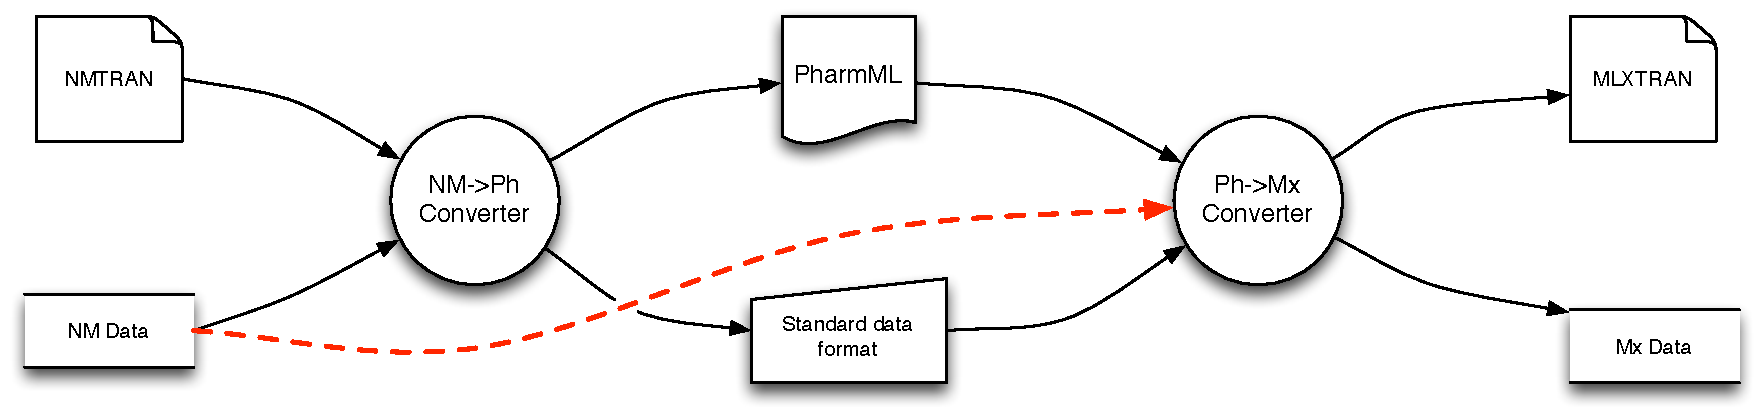
\includegraphics[width=\linewidth]{DataConversion}
\caption{Converting model and data to \pharmml. The figure shows how
  the NONMEM to \pharmml (NM$\rightarrow$Px) converter must convert both the
  model and data and then the \pharmml to MONOLIX (Ph$\rightarrow$Mx) converter
  must convert the \pharmml and standard data files to the MLXTRAN and a
  MONOLIX formatted data file.}
\label{fig:data-conversion}
\end{figure}

This approach undoubtedly requires more work on the part of the
converter generating \pharmml because it must also do the data format
conversion too. However, I would argue that this makes sense because
the developer and maintainer of this converter will of necessity be
very familiar with the tool and so will be familiar with its data
format. Without converting to the standard data format then the
situation illustrated by the red line in figure \ref{fig:data-conversion}
will occur. Here the converter that translates from \pharmml will need
to understand NONMEM data format and convert it into MONOLIX data
format. However, this converter would also need to be able to convert
CVS, TSV, and WinBugs formats too. Clearly this is a lot of work and
it is unlikely that the development and maintenance team will be
closely familiar with these formats. By converting to a standard data
format, however, we can avoid these problems and we can focus our
efforts on providing a software library to wrote and read this
format.

If we wish to adopt a standard data format, what should it be? We
could design our own, but it would make sense to use an existing
standard that is designed for this purpose. My candidate is
NuML\footnote{\url{http://http://code.google.com/p/numl/}}. This
originated from a Systems Biology related format (SBRML) that was
designed to store the results of a simulation\footnote{See also:
  \url{http://www.comp-sys-bio.org/tiki-index.php?page=SBRML}}. It
will hold the tabular data we wish to use for estimation in \pharmml,
but it should also be able to store results generated by estimation
and simulations defined in \pharmml. Since capturing the results of
such tasks is within the scope of \pharmml this allows us to
standardise on one data format for all our needs. Software support is
available in C++ and Java (not native Java) too and there is an XML
Schema that we would be able to reuse directly within \pharmml. We
could therefore embed NuML data directly in the \pharmml file or link
to it as an external file.

\subsubsection{Conclusion}

\watchout There has not been time to investigate how NuML can be used. A problem
was also identified when re-factoring the trial design in that it
seems that NuML cannot handle multi-dimensional data in the way that
\pharmml requires. This area needs more work, but for the moment we
are using a revised version of the \xelem{Dataset} structured found in
version 0.1 of \pharmml (see section \ref{sec:dataset-refactoring}).

\section{Changes agreed}

\subsection{Revise the XML design principles used}

A common dilemma when designing XML documents is when do I use an
element and when an attribute? Previously when designing \pharmml we
have tended to use attributes to hold information. However, some of
these usages are at odds with design best practise, such as the guidelines provided in an IBM technical
document\footnote{\url{http://http://www.ibm.com/developerworks/xml/library/x-eleatt/index.html}}. The
advice can be summarised as follows:

\begin{description}
\item[Principle of core content] Briefly data or core content should
  be held in elements and metadata should be in attributes.
\item[Principle of structured information] If the information needs to
  be structured then it should be represented by an element. If it is
  atomic then us an attribute.
\item[Principle of readability] If the information is intended to be
  read and understood by a person then use elements. If it is intended
  to be used by a machine then use attributes.
\item[Principle of element/attribute binding] If the information to be
  represented can be modified by another attribute then use an element
  to represent it.
\end{description}

These rules are to some extent a matter of judgement and in some cases
it is not immediately clear what constitutes core content or
metadata. The names of parameters, variables and other symbols used in
\pharmml are a case in point. The names for such symbols have meaning
for a modeller, but they are also used computationally to validate the
\pharmml document. In addition, variable names can have two forms: a
computer friendly form such as \texttt{omega\_V} and a mathematical
form such as $\omega_V$. Currently \pharmml only handles the latter
form, and although this is a computational name it is also the
variable name commonly used by modellers. So if the computational name
is also the name used when discussing a model is it worth
distinguishing between the two? My proposal is to
define the identifier that is used computationally as an attribute,
but to also provide an optional `publishable' symbol name as an element. That way if
it is useful to make a distinction you can, otherwise the
computational identifier can be used as the publishable name for the
symbol. For example:
%
\begin{xmlcode}
<Variable symbID="pV" symbolType="scalar" >
  <ct:Symbol>pop_V</Symbol>
</Variable>
\end{xmlcode}

Another area where applying these design guidelines changes things is
in the way we represent numbers and other similar constructs. Instead
of using a
\xatt{value} attribute we define it using element content. So the
following:
%
\begin{xmlcode}
<ct:Scalar value="10.1"/>
<ct:Sequence begin="0" end="192" stepSize="24" />
<ct:Sequence begin="0" repetitions="2" stepSize="24" />
<ct:String value="foo"/>
\end{xmlcode}
%
becomes
%
\begin{xmlcode}
<ct:Scalar>10.1</ct:Scalar>
<ct:Sequence>
    <ct:Begin>0</ct:Begin>
    <ct:StepSize>24</ct:StepSize>
    <ct:End>192</ct:End>
</ct:Sequence>
<ct:Sequence>
    <ct:Begin>0</ct:Begin>
    <ct:StepSize>24</ct:StepSize>
    <ct:Repetitions>2</ct:Repetitions>
</ct:Sequence>
<ct:String>foo</ct:String>
\end{xmlcode}

Note that in the case of the sequence the new construct also allows us
to ensure that only a repetition or an end is defined. With the
attribute approach above this could not be validated by XML Schema
validation.


\subsection{Define basic types in common types}

Currently types like \xelem{Scalar} and \xelem{VarRef} are define in
the maths schema. While this works, it make the design a messy as the
original concept was that the maths schema was an separate module
independent of the rest of the schema. The aim of making it modular
was to make sure we could minimise the impact of replacing our maths
definition with another definition, such as MathML should we wish
to\footnote{Likewise the Uncertainty schema that describes probability
  distributions is also modular so that we can replace it by UncertML
  version 3.0.}.

The proposal is that we define the basic types such as string,
scalar\footnote{See later proposal about numerical types.} and
Booleans as common types.


\subsection{Different Numerical Types}

Currently there is a single type for a number called the scalar. The
idea is that a scalar type can be any numerical value and the term
scalar is used to distinguish it from an array type (which we don't
have, but could do it in the future). However, in some cases it is
useful to distinguish between integer and real numbers in
\pharmml. For example, when defining a sequence the number of
repetitions should be an integer (actually a positive integer) or when
specifying the number of individuals in a Trial Design Group.

My proposal is that we have two numerical literal elements \xelem{Int}
and \xelem{Real}. These would work as follows:

\begin{xmlcode}
<ct:Int>10</ct:Scalar>
<ct:Int>-210</ct:Scalar>
<ct:Real>22.2</Real>
<ct:Real>1.5636e-36</ct:Real>
<ct:Real>.0273626</ct:Real>
<ct:Real>-2.03</ct:Real>
<ct:Real>INF</ct:Real>
\end{xmlcode}

There is a question whether we should define the element as
\xelem{Double} instead of \xelem{Real}. Ideally the \xelem{Real}
element would define an architecture independent real number with
arbitrary precision. However, applications that use such numbers will
typically use a double numerical type. Therefore we should define the
\xelem{Real} element to be an XML Schema double type, which conforms
to the IEEE double-precision 64-bit floating point type standard used
by many programming languages. This begs the question of whether we
should rename the \xelem{Real} element to be \xelem{Double} as this
matches the computational representation of the number and so makes it
clear to the user of \pharmml. An argument against this is that we are
only providing one Real type; so we don't need to distinguish between
a double and a float for example. Likewise, if we decide to change the
underlying type of \xelem{Real}, for example from double to a float,
then this change would not require a change at the XML level and the
name would not be mislead, as it would if we called the element
\xelem{Double}. On balance my preference is to use the element name
Real.

\subsubsection{Conclusion}

A Real and Int type has been added to schema. Note that we will
introduce a system of type promotion when type checking. \watchout Simply put
this means that an integer can be converted to a real number on the
fly, but the reverse is not permitted and will give a type checking error.

\subsection{Change Variability Levels to be Declarative}

Currently the order of a variability level definition is used to
specified the hierarchy of variability levels. So for example to
define BSV and IOV we define the IOV level first then the BSV level
next, as below:
%
\begin{xmlcode}
<VariabilityLevel id="iov1"/>
<VariabilityLevel id="indiv"/>
\end{xmlcode}

As was pointed out by Duncan Edwards this is actually an imperative
definition as the ordering the elements are read in is important. He
suggested we make the hierarchy definition explicit and on reflection
I think he is right. Therefore I propose we change the definition to
the following:
%
\begin{xmlcode}
<VariabilityModel id="model">
    <Level symbId="indiv"/>
    <Level symbId="iov1">
        <ParentLevel>
            <ct:SymbRef symbId="indiv"/>
        </ParentLevel>
    </Level>
</VariabilityModel>
\end{xmlcode}

Here each level defines it's parent level explicitly and the topmost
level has no parent defined. It is important to note that the order is
now not significant so the following definition is equivalent to the
one above:
%
\begin{xmlcode}
<VariabilityModel id="model">
    <Level symbId="iov1">
        <ParentLevel>
            <ct:SymbRef symbId="indiv"/>
        </ParentLevel>
    </Level>
    <Level symbId="indiv"/>
</VariabilityModel>
\end{xmlcode}
%
The other thing to note is that the variability levels are now held in
a block. This is consistent with the other models in
\xelem{ModelDefinition} and this feature may be useful later when we
think about defining the variability of the residual error model.

\subsection{Improving the definition of a variable}

Applying the attribute/element design guidelines above we can refactor
the way a variable definition is designed in \pharmml. There are two main
changes. One is the way we define derivative variables (see below) and
the other is the way we indicate assignment. The example below shows the
changes:
%
\begin{xmlcode}
<ct:Variable symbId="k" symbolType="real">
    <ct:Symbol>k</ct:Symbol>
    <ct:Description>This is a description.</ct:Description>
    <ct:Assign>
        <Equation xmlns="http://www.pharmml.org/2013/03/Maths" writtenVersion="0.1">
            <Binop op="divide">
                <Var block="p1" symbId="Cl"/>
                <Var block="p1" symbId="V"/>
            </Binop>
        </Equation>
    </ct:Assign>
</ct:Variable>
\end{xmlcode}
%
The \xelem{Symbol} and \xelem{Description} elements are optional. We
use an \xelem{Assign} element to indicate where the RHS of the
assignment is. This is optional --- a variable does not need to be
assigned when it is defined. We could strictly do without the
\xelem{Assign} element but it makes the design cleaner and reduces
redundancy as we reference a global \xelem{Assign} element defined in
the Common Types schema. This makes it simpler to parse the model as standard
syntactic patterns are reused throughout the language.

\subsection{Improving the definition of a derivative}

Currently we use the type to define whether a variable is a
derivative. While this works it is not strictly correct as the type of
the variable is a scalar \emph{and} the variable is also a
derivative. While at the moment this does not matter, the current
approach is not easily extensible. For example it may be useful in the
future to provide derivatives for variables with types not yet
supported, such as vectors. In addition, the independent variable is
defined as an attribute that should only be defined if the variable is
a derivative. This is a rule that cannot be enforced by XML schema
validation directly. However, after refactoring to an element is can
be. The example below shows the current approach:
%
\begin{xmlcode}
<Variable symbId="x" independentVar="t" symbolType="derivative">
    <Equation xmlns="http://www.pharmml.org/2013/03/Maths" writtenVersion="0.1">
      <!-- Snip -->
    </Equation>
</Variable>
\end{xmlcode}
%
and how the same definition would look under this proposal:
%
\begin{xmlcode}
<ct:DerivativeVariable symbId="x" symbolType="real">
    <ct:Description>Concentration</ct:Description>
    <ct:Assign>
        <Equation xmlns="http://www.pharmml.org/2013/03/Maths" writtenVersion="0.1">
          <!-- Snip -->
        </Equation>
    </ct:Assign>
    <ct:IndependentVariable>
        <ct:SymbRef symbId="t"/>
    </ct:IndependentVariable>
    <ct:InitialCondition>
       <ct:Real>0</ct:Real>
    </ct:InitialCondition>
</ct:DerivativeVariable>
\end{xmlcode}

By using the \xelem{ct:DerivativeVariable} element we can now enforce
the rule that the independent variable can only be defined for a
derivative variable. Note that the type of the variable is defined
using the \xatt{symbolType} attribute, which has it's value fixed to
`real'. We do this because \pharmml only supports derivative variables
of that type, but providing the attribute enables future modification
and makes the XML self-documenting. The final change of note is that
the initial condition is now associated with the
derivative. Previously this was a completely separate element, but by
making it part of the derivative we ensure that only derivative
variables are provided with initial conditions.

\subsection{Improving the definition of a variable assignment}

The refactoring of the assignment follows the element vs attribute
design principle described above and aims to be consistent with the
variable declaration. See the example:
%
\begin{xmlcode}
<ct:VariableAssignment>
    <ct:SymbRef  block="c1" symbId="omega_W"/>
    <ct:Description>This is the: c1.omega_W = 1409/100</ct:Description>
    <ct:Assign>
        <math:Equation writtenVersion="0.1">
            <!-- 1409/100 = 14.09 -->
            <math:Binop op="divide">
                <math:Scalar>1409</math:Scalar>
                <math:Scalar>100</math:Scalar>
            </math:Binop>
        </math:Equation>
    </ct:Assign>
</ct:VariableAssignment>
\end{xmlcode}
%
The \xelem{VariableAssignment} is defined as a common type and is
reused in several places throughout the schema.

\subsection{Reusing common elements}

In the current version of \pharmml we have a schema called
commonTypes.xsd where we put commonly used types such as variable
references, sequences, vectors etc. The idea is that this schema holds
common types and structures that are used in common by the other
schemas (except Math.xsd and Uncertainty.xsd). This helps us remove
redundancy in the design and makes changing and extending the schema
easier. During the refactoring I propose to extend this approach and
put reusable elements into the common schema. Elements such as String,
SymbRef, VariableAssignment etc are defined here as global elements
that can then be referenced by the other schemas. In addition to
further reducing redundancy this approach also promotes the reuse of
the same constructs throughout the language which simplifies parsing
and validation of the language.

To help with this some elements in the current \pharmml spec are being
replaced with a common reference. In particular the
\xelem{initialAssignment} element in the simulation and estimation
step is being replaced with a reference to the
\xelem{VariableAssignment} element and the variable declarations in
the \xelem{ModellingSteps} and \xelem{StructuralModel} elements are
each replaced by the VariableAssignment.


\subsection{Element identifier for annotation?}
\label{sec:id-prop}

Our current idea of how to link annotation (aka metadata) to a
\pharmml document is to use xpath to point from the ontology terms to
the elements in the XML document. While this will work and be very
flexible I am not clear how we will be able to map from the XML
structures identified to the software API. For example, if we want to
annotate a variable definition the xpath definition would identify the
\xelem{VariableDefinition} element containing this definition. In
software we would need to find this element in the XML and then map
from this element to a corresponding Java class in libPharmML. This
may be possible, but an alternate way to do the same thing would be to
write an xpath that points to the \xatt{symbID} attribute of the same
element. Getting the software to recognise that these are essentially
the same may be difficult. We need to explore this by testing to be
sure, but an alternate mechanism may be to provide all elements with a
unique identifier, an \xatt{id} attribute. If this was mandatory for
all elements then you could guarantee that all elements in the
\pharmml document are annotatable. The \xatt{id} would also be an
attribute in the Java class so the mapping between annotation and
PharmML could be carried out directly at the software level. This is a
stricter form of the approach taken by SBML, which uses a
\xatt{metaid} attribute that is optional. SBML uses \xatt{metaid}
because the \xatt{id} attribute was originally used to define variable
names. The \xatt{id} convention is consistent with other XML schemes
such as MathML and XML-RDF. Making it mandatory means that we don't
have to change the \pharmml document in order to annotate it, because
all elements are guaranteed to have an identifier that can be
referenced. Incidentally, this approach will be much more effective
after the refactoring ideas described above are implemented because
the elements of information that we may want to annotate are stored as
XML elements whereas in some cases they are currently represented as
XML attributes.

Below is a code snippet illustrating how this identifier would work:

\begin{xmlcode}
<FixedEffect id="e10" symbId="beta_V">
    <Covariate id="e11" >
        <ct:SymbRef id="e12" symbId="W"/>
    </Covariate>
</FixedEffect>
<FixedEffect id="e13" symbId="beta_Cl">
    <Covariate id="e14">
        <ct:SymbRef id="e15" symbId="W"/>
    </Covariate>
</FixedEffect>
<RandomVariable id="e16" symbId="eta_V">
    <ct:VariabilityReference id="e17">
        <ct:SymbRef id="e18"  block="model" symbId="level"/>
   </ct:VariabilityReference>
\end{xmlcode}

\subsubsection*{Conclusion}

Added to all elements in the schema\footnote{Well nearly all. I need
  to test this.}. I have made the \xatt{id} optional for the moment.

\subsection{Improved Parameter Model}

In the previous proposal I outlined a change to the definition of the
parameter model. The change was to remove assumptions from the
parameter definition and thus to allow parameter definitions that were
not permitted in version 0.1 of the specification. Feedback about this
was generally positive, except Mark Lavielle who felt that this
definition was  a step backwards because we lots the description of
the components of the parameter definition. His proposal was to
define the parameter using one of the following forms:

\begin{align*}
\intertext{Type 1. (implicit) equation type of parameter model}
\psi_i &= H(\beta, c_i, \eta_i)
\intertext{Type 2. Gaussian model with general covariate model}
h(\psi_i) &= H(\beta, c_i) + \eta_i
\intertext{Type 3. Gaussian model with linear covariate model}
h(\psi_i) &= h(\psi_{pop}) + \beta c_i + \eta_i
\end{align*}
with:
\begin{itemize}
\item individual parameter, $\psi_i$
\item population parameter, $\psi_{\textit{pop}}$
\item random effect, $\eta_i$
\item fixed effects, $\beta$
\item arbitrary function , $H$
\item function which transforms the model on both sides, $h$
\end{itemize}

Using these definitions form 3 corresponded to the parameter
definition used in version 0.1\footnote{Well in fact that's almost
  correct. On closer description we found that in version 0.1 we did not explicitly
  constrain ,$h$, the transformation, to be the same on both sides of
  the equation.} and form 1 to the form described in the
previous proposal. Therefore I have updated the parameter definition
to incorporate the three forms above. This should provide total
flexibility, but also make it possible for tools that care to use the
most structures parameter definitions (forms 2 and 3).

As a consequence of the this, the Parameter definition has become more
complicated as we also permit simple parameters definitions, which may
or may not be initialised as well as the individual parameters
definitions above. Therefore in this proposal I have split these
representations between \xelem{SimpleParameter} and
\xelem{IndividualParameter} elements.

Below are some examples:

\subsubsection{Type 1: Implicit definition}

This might be thought of as the typical way a parameter is defined in NONMEM.

\begin{align*}
V_i &= \mathrm{pop}_{V} \left(\frac{W_{i}}{70}\right)^{\beta_{V}} e^{\left(\eta_{V_i} \right)}
\end{align*}
%
and this can now be encoded, without transformation, as:
%
\begin{xmlcode}
<SimpleParameter symbId="pop_V"/>
<SimpleParameter symbId="omega_V"/>
<SimpleParameter symbId="beta_V"/>
<RandomVariable symbId="eta_V">
    <ct:VariabilityReference>
        <ct:SymbRef block="model" symbId="indiv"/>
    </ct:VariabilityReference>
    <NormalDistribution xmlns="http://www.uncertml.org/3.0" definition="">
        <mean><rVal>0</rVal></mean>
        <stddev><var varId="omega_V"/></stddev>
     </NormalDistribution>                            
 </RandomVariable>
<IndividualParameter symbId="V">
    <ct:Assign>
        <Equation xmlns="http://www.pharmml.org/2013/03/Maths">
            <Binop op="times">
                <ct:SymbRef symbId="pop_V"/>
                <Binop op="times">
                    <Binop op="pow">
                        <Binop op=''divide''>
                            <ct:SymbRef block="c1" symbId="W"/>
                            <ct:Real>70</ct:Real>
                        </Binop>
                        <ct:SymbRef symbId="beta_V"/>
                    </Binop>
                    <Uniop op="exp">
                        <Var symbId="eta_V"/>
                    </Uniop>
                </Binop>
            </Binop>
        </Equation>
    </ct:Assign>
</IndividualParameter>
\end{xmlcode}

Note that this version uses the prototype of \uncertml 3.0.

\subsubsection{Type 2: Gaussian Model with General Covariate Model}

The following is modified from the NONMEM User Manual\footnote{NONMEM
  Users Guide - Part V: Introductory Guide, p 34.}  and describes an
individual parameter with a non-linear covariate model as follows:
%
\begin{align*}
\mathrm{CL} &= W \left(\Theta_1 -
  \left(\frac{\Theta_2 \mathrm{Cpss_2}}{\Theta_3 +
      \mathrm{Cpss}_2}\right)\right) + \eta_{\mathrm{CL}}
\end{align*}
%
We can express this using the general covariate form of the parameter model as follows: 
%
\begin{xmlcode}
<IndividualParameter symbId="CL">
    <GaussianModel>
        <GeneralCovariate>
            <Assign xmlns="http://www.pharmml.org/2013/03/CommonTypes">
                <Equation xmlns="http://www.pharmml.org/2013/03/Maths"
                    writtenVersion="0.1">
                    <Binop op="times">
                        <Var block="c1" symbId="W"/>
                        <Binop op="minus">
                            <Var symbId="theta1"/>
                            <Binop op="divide">
                                <Binop op="times">
                                    <Var symbId="theta2"/>
                                    <Var symbId="Cpss2"/>
                                </Binop>
                                <Binop op="plus">
                                    <Var symbId="theta3"/>
                                    <Var symbId="Cpss2"/>
                                </Binop>
                            </Binop>
                        </Binop>
                    </Binop>
                </Equation>
            </Assign>
        </GeneralCovariate>
        <RandomEffects>
            <ct:SymbRef symbId="eta_CL"/>
        </RandomEffects>
    </GaussianModel>
</IndividualParameter>
\end{xmlcode}


\subsubsection{Type 3: Gaussian Model with Linear Covariate}

This is the form familiar from version 0.1 or the \pharmml specification:
%
\begin{align}
\log(V_i) &= \log(\mathrm{pop_{V}}) + \beta_{1,V}\log(W_i/70) + \eta_{V,i}
\end{align}
%
We define this in XML by defining the fixed effect parameters, the random
variable and then the parameter which incorporates these elements into
the above equation.
%
\begin{xmlcode}
<SimpleParameter symbId="beta_V"/>
<SimpleParameter symbId="pop_V"/>
<SimpleParameter symbId="omega_V"/>
<RandomVariable symbId="eta_V">
    <ct:VariabilityReference>
       <ct:SymbRef block="model" symbId="level"/>
    </ct:VariabilityReference>
    <NormalDistribution xmlns="http://www.uncertml.org/3.0" definition="">
        <mean><rVal>0</rVal></mean>
        <stddev><var varId="omega_V"/></stddev>
    </NormalDistribution>                            
</RandomVariable>
<IndividualParameter symbId="V">
    <GaussianModel>
        <Transformation>log</Transformation>
        <LinearCovariate>
            <PopulationParameter>
                <ct:Assign>
                    <ct:SymbRef symbId="pop_V"></ct:SymbRef>
                </ct:Assign>
            </PopulationParameter>
            <Covariate>
                <ct:SymbRef block="c1" symbId="W"></ct:SymbRef>
                <FixedEffect>
                    <ct:SymbRef symbId="beta_V"></ct:SymbRef>
                </FixedEffect>
            </Covariate>
        </LinearCovariate>
        <RandomEffects>
            <ct:SymbRef symbId="eta_V"></ct:SymbRef>
        </RandomEffects>
    </GaussianModel>
</IndividualParameter>
\end{xmlcode}

\paragraph{The covariate model: incorporating categorical covariates}

A benefit of this approach is that we can revert to dealing with
categorical covariates in the same way as we do in the current version
of the specification, which is clearer and more explicit. So we can
encode:
%
\begin{align*}
1_{\mathrm{ka,TreatSeq}_i=\mathrm{A-B}} &=
\begin{cases}
1 & \text{if } W \text{ has category } \mathrm{A-B}\\
0 & \text{otherwise}
\end{cases}
\intertext{We can incorporate this into the full parameter definition:}
\log(ka_{i}) &= \log(ka_{pop}) + \beta_{ka,TreatSeq}1_{TreatSeq_i=\mathrm{A-B}} + \eta_{ka,i}
\end{align*}
%
as:
%
\begin{xmlcode}
<Parameter symbId="one_ka_treatseq">
    <ct:Symbol>1_ka_treatset</ct:Symbol>
    <ct:Assign>
        <math:Equation writtenVersion="0.1">
            <math:Piecewise>
                <math:Piece>
                    <math:Scalar>1</math:Scalar>
                    <math:Condition writtenVersion="0.1">
                        <math:LogicBinop op="eq">
                            <math:Var block="c1" symbId="W"/>
                            <math:String value="AB"/>
                        </math:LogicBinop>
                    </math:Condition>
                </math:Piece>
                <math:Piece>
                    <math:Scalar>0</math:Scalar>
                    <math:Condition writtenVersion="0.1">
                        <math:Otherwise/>
                    </math:Condition>
                </math:Piece>
            </math:Piecewise>
        </math:Equation>
    </ct:Assign>
</Parameter>
\end{xmlcode}

\subsubsection{We still retain flexibility}

Just to emphasise the point, all models that were encodable in the
previous proposal are still encodeable. This is the example used in
the previous proposal of an individual parameter definition,
I've taken from Hooker \emph{et al.} 2008\footnote{ Hooker
  et al. ``Population Pharmacokinetic Model for Docetaxel in Patients
  with Varying Degrees of Liver Function: Incorporating Cytochrome
  P450 3A Activity Measurements'' Clinical Pharmacology \& Therapeutics
  84, 111-118 (July 2008) \textbar
  \url{doi:10.1038/sj.clpt.6100476}}. We describe unbound plasma
clearance using the individual parameter $\mathit{CL}_i$ as follows:
%
\begin{align*}
\mathrm{CL}_i &=
\begin{cases}
\eta_{\mathrm{CL}} \cdot \mathrm{CL}_{\mathrm{normal\, LF}} \cdot f_{\mathrm{BSA}} \cdot
f_{\mathrm{AAG}} \cdot f_{\mathrm{ERMBT, normal\, LF}} & \text{if } \mathrm{LFG} = 1\\
\eta_{\mathrm{CL}} \cdot \mathrm{CL}_{\mathrm{impaired\, LF}} \cdot f_{\mathrm{BSA}} \cdot
f_{\mathrm{AAG}} \cdot f_{\mathrm{ERMBT, impaired\, LF}} & \text{if } \mathrm{LFG}
> 1
\end{cases}\\
f_{\mathrm{BSA}} &= \mathrm{BSA} / \overline{\mathrm{BSA}}\\
f_{\mathrm{AAG}} &= 1 + \theta_{\mathrm{AAG-CL}} \cdot \left(\mathrm{AAG} / \overline{\mathrm{AAG}}\right)\\
f_{\mathrm{ERMBT, normal\, LF}} &= 1 + \theta_{\mathrm{ERMBT, normal\, LF}} \cdot
\left(\mathrm{ERMBT} - \overline{\mathrm{ERMBT}}_{\mathrm{normal\, LF}}\right)\\
f_{\mathrm{ERMBT, impaired\, LF}} &= 1 + \theta_{\mathrm{ERMBT, impaired\, LF}} \cdot
\left(\mathrm{ERMBT} - \overline{\mathrm{ERMBT}}_{\mathrm{impaired\, LF}}\right)
\end{align*}
%
With the proposed changes to the paramater model this can be encoded
as follows:
%
\begin{xmlcode}
<SimpleParameter symbId="f_ERMBT_normalLF">
    <ct:Assign>
        <Equation xmlns="http://www.pharmml.org/2013/03/Maths" writtenVersion="0.1">
            <Binop op="plus">
                <Scalar>1</Scalar>
                <Binop op="times">
                    <Var symbId="theta_ERMBT_normalLF"/>
                    <Binop op="minus">
                        <Var symbId="ERMBT"/>
                        <Var symbId="ERMBT_normalLF"/>
                    </Binop>
                </Binop>
            </Binop>
        </Equation>
    </ct:Assign>
</SimpleParameter>
<Parameter symbId="theta_ERMBT_impairedLF"/>
<SimpleParameter symbId="f_ERMBT_impairedLF">
    <ct:Assign>
        <Equation xmlns="http://www.pharmml.org/2013/03/Maths" writtenVersion="0.1">
            <Binop op="plus">
                <Scalar>1</Scalar>
                <Binop op="times">
                    <Var symbId="theta_ERMBT_impairedLF"/>
                    <Binop op="minus">
                        <Var symbId="ERMBT"/>
                        <Var symbId="ERMBT_impairedLF"/>
                    </Binop>
                </Binop>
            </Binop>
        </Equation>
    </ct:Assign>
</SimpleParameter>
<SimpleParameter symbId="theta_AAG_CL"/>
<SimpleParameter symbId="f_AAG">
    <ct:Assign>
        <Equation xmlns="http://www.pharmml.org/2013/03/Maths" writtenVersion="0.1">
            <Binop op="plus">
                <Scalar>1</Scalar>
                <Binop op="times">
                    <Var symbId="theta_AAG_CL"/>
                    <Binop op="minus">
                        <Var symbId="AAG"/>
                        <Var symbId="AAG_bar"/>
                    </Binop>
                </Binop>
            </Binop>
        </Equation>
    </ct:Assign>
</SimpleParameter>
<SimpleParameter symbId="f_BSA">
    <ct:Assign>
        <Equation xmlns="http://www.pharmml.org/2013/03/Maths" writtenVersion="0.1">
            <Binop op="divide">
                <Var symbId="BSA"/>
                <Var symbId="BSA_bar"/>
            </Binop>
        </Equation>
    </ct:Assign>
</SimpleParameter>
<RandomVariable symbId="eta_CL">
    <ct:VariabilityReference>
        <ct:SymbRef symbId="indiv"/>
    </ct:VariabilityReference>
    <Distribution xmlns="http://www.pharmml.org/2013/03/Uncertainty"
    writtenVersion="0.1">
         <!-- Snip -->
    </Distribution>
</RandomVariable>
<IndividualParameter symbId="CL">
    <ct:Assign>
        <Equation xmlns="http://www.pharmml.org/2013/03/Maths" writtenVersion="0.1">
            <Piecewise>
                <Piece>
                    <Binop op="times">
                        <Uniop op="exp"><Var symbId="eta_CL"/></Uniop>
                        <Binop op="times">
                            <Var symbId="CL_normalLDF"/>
                            <Binop op="times">
                                <Var symbId="f_BSA"/>
                                <Binop op="times">
                                    <Var symbId="f_AAG"/>
                                    <Var symbId="f_ERMBT_normalLF"/>
                                </Binop>
                            </Binop>
                        </Binop>
                    </Binop>
                    <Condition writtenVersion="0.1">
                        <LogicBinop op="eq">
                            <Var symbId="LFG"/>
                            <Scalar>1</Scalar>
                        </LogicBinop>
                    </Condition>
                </Piece>
                <Piece>
                    <Binop op="times">
                        <Uniop op="exp">
                            <Var symbId="eta_CL"/>
                        </Uniop>
                        <Binop op="times">
                            <Var symbId="CL_impairedLF"/>
                            <Binop op="times">
                                <Var symbId="f_BSA"/>
                                <Binop op="times">
                                    <Var symbId="f_AAG"/>
                                    <Var symbId="f_ERMBT_impairedLF"/>
                                </Binop>
                            </Binop>
                        </Binop>
                    </Binop>
                    <Condition writtenVersion="0.1">
                        <LogicBinop op="gt">
                            <Var symbId="LFG"/>
                            <Scalar>1</Scalar>
                        </LogicBinop>
                    </Condition>
                </Piece>
            </Piecewise>
        </Equation>
    </ct:Assign>
</individualParameter>
\end{xmlcode}


This example highlights an important question. When is a parameter an
\xelem{IndividualParameter} or a \xelem{SimpleParameter}. If the
equation includes a random variable then you should use the
\xelem{IndividualParameter} element. This is something we could
enforce as a rule within the specification.


\subsection{Add variability levels to the observation model}

Currently the observation model can only contain one level of
variability that is defined implicitly. At the consortium meeting and
in subsequent discussions with others, including NH, there is a strong
feeling was that we needed a to be able to define a residual error
model with multiple levels of variability. My initial idea had been to
replicate the variability level structures used in the
\xelem{ModelDefinition} in the \xelem{ObservationsModel}, but this
didn't fit in with the refactored \xelem{VariabilityModel}
proposal. So the best approach is to define a single
variability hierarchy definition. This is consistent with the way MDL
does things and it also is the most flexible approach that avoids
making any assumptions that we may need to undo later. However,
because the \xelem{VariabilityModel} now uses the block structure and
has its own block identifier we can take advantage of this to separate
out the definitions for the residue error variability and the model
variability. This is illustrated in the example below:

\begin{xmlcode}
<ModelDefinition>
    <VariabilityModel id="model">
        <Level symbId="indiv">
            <ct:Name>Individual Variability</ct:Name>
        </Level>
    </VariabilityModel>
    <VariabilityModel id="obsErr">
        <Level symbId="residual">
            <ct:Name>Residual Error</ct:Name>
            <ParentLevel>
                <ct:SymbRef block="model" symbId="indiv"/>
            </ParentLevel>
        </Level>
    </VariabilityModel>
    <!-- 
       The covariate, parameter and structural model are omitted. Look at
       example1.xml for the full example.
       -->
    <ObservationModel id="o1">
        <Continuous symbId="Cc">
            <RandomVariable symbId="epsilon_Cc">
                <ct:VariabilityReference>
                    <ct:SymbRef block="obsErr" symbId="residual"/>
                </ct:VariabilityReference>
                <Distribution xmlns="http://www.pharmml.org/2013/03/Uncertainty"
                    writtenVersion="0.1">
                    <Normal>
                        <Mean>
                            <Equation xmlns="http://www.pharmml.org/2013/03/Maths"
                                writtenVersion="0.1">
                                <math:Scalar>0</math:Scalar>
                            </Equation>
                        </Mean>
                        <StdDev>
                            <Equation xmlns="http://www.pharmml.org/2013/03/Maths"
                                writtenVersion="0.1">
                                <math:Scalar>1</math:Scalar>
                            </Equation>
                        </StdDev>
                    </Normal>
                </Distribution>
            </RandomVariable>
            <ct:Assign>
                <math:Equation writtenVersion="0.1">
                    <math:Binop op="plus">
                        <math:Var block="main" symbId="Cc"/>
                        <math:Binop op="times">
                            <math:FunctionCall>
                                <math:Var symbId="combinedErrorModel"/>
                                <math:FunctionArgument symbId="a">
                                    <math:Var symbId="a1"/>
                                </math:FunctionArgument>
                                <math:FunctionArgument symbId="b">
                                    <math:Var symbId="b1"/>
                                </math:FunctionArgument>
                                <math:FunctionArgument symbId="f">
                                    <math:Equation writtenVersion="0.1">
                                        <math:Var block="main" symbId="Cc"/>
                                    </math:Equation>
                                </math:FunctionArgument>
                            </math:FunctionCall>
                            <math:Var symbId="epsilon_Cc"/>
                        </math:Binop>
                    </math:Binop>
                </math:Equation>
            </ct:Assign>
        </Continuous>
    </ObservationModel>
</ModelDefinition>
\end{xmlcode}

As is described above the \xelem{RandomVariable} element refers to a
variability level. You can see this by looking at the \xatt{obsErr}
random variable, which contains a reference to the \xatt{residual}
variability level that is define in the \xatt{obsErr} variability
model. In other words the residual error variability level
is now explicit rather than implicit as it is in the current release
of \pharmml. In addition it is now possible to have multiple levels of
variability in the residual error model.

By putting the residue error variability in a \xelem{VariabilityModel}
with the id 'obsErr' that is separate to the 'model' variability
model, we can make a clear distinction between what is the residual
error model variability and what is the 'model' variability. However,
the important thing to note is that this is just a \emph{convention}
that you can use to make the model clearer. We could have define the
variability model in one block as follows:
%
\begin{xmlcode}
<VariabilityModel id="model">
    <Level symbId="indiv">
        <ct:Name>Individual Variability</ct:Name>
    </Level>
    <Level symbId="residual">
        <ct:Name>Residual Error</ct:Name>
        <ParentLevel>
            <ct:SymbRef symbId="indiv"/>
        </ParentLevel>
    </Level>
</VariabilityModel>
\end{xmlcode}
%
and this would have been equivalent to the earlier example.  The
important point is that both code snippets define the same variability
level hierarchy. The intent of the first one is just clearer because
we define it using two variability model blocks.

\subsection{Units}

A restricted version of the SBML approach looks like it should work in
\pharmml. The question is should we add in units now? The approach
would be to have a built-in set of fundamental units that cover all
dimensions. Then you could define specific units based on these
conventions. For example we may have a $g$ as the fundamental unit of
mass and then define a $kg$ which is a gram scaled by 1000. An example
of what it might look like is below:
%
\begin{xmlcode}
<UnitDefinition symbId="hour">
    <Symbol>h</Symbol>
    <Unit basicUnit="second">
        <Exponent>1</Exponent>
        <Scale>1</Scale>
        <Multiplier>60</Multiplier>
    </Unit>
</UnitDefinition>
\end{xmlcode}
%
The \xelem{UnitDefinition} element defines the unit in terms of a base
unit referred to in the \xelem{Unit} element. Following advice from
Sarah Keating of the SBML team, and the developer who has implemented
unit checking in libSBML, we should keep the set of basic units as
minimal as possible. In this example the idea would be to use the
seven base units from SI\footnote{See Section 2 in
  \url{http://http://www.bipm.org/utils/common/pdf/si_brochure_8.pdf}.}.
The \xelem{Unit} element describes the conversion of the base
unit a consistent of the unit being defined. In this case the unit \emph{hour} is defined
as 60 seconds.

More complex units can contain multiple \xelem{Unit}
elements:
%
\begin{xmlcode}
<UnitDefinition symbId="velocity">
    <ct:Symbol>ms-1</ct:Symbol>
    <Unit basicUnit="metre">
        <Exponent>1</Exponent>
    </Unit>
    <Unit basicUnit="second">
        <Exponent>-1</Exponent>
    </Unit>
</UnitDefinition>
\end{xmlcode}

Above we define velocity, $ms^{-1}$. Note that if the \xelem{Scale}
and \xelem{Multiplier} elements are omitted they are assumed to be
1. The example below shows how we might use these definitions, for
example to define the time units used in the model:
%
\begin{xmlcode}
<IndependentVariable symbId="t">
    <Units symbId="hour"/>
</IndependentVariable>
\end{xmlcode}

Our advice is that the key thing is to put units on all quantities,
including numbers, that was unit consistency checking should be
straightforward as then no inference is required. \pharmml already has
a type system which we need to check for consistency anyway. This
helps here, because units can be thought of as another set of types
and so we should be able to extend the type checking system to
validate unit consistency. My suggestion would be to put in the
structures we need for units now, but only add validation rules about
unit consistency checking later.

\subsubsection{Conclusion}

\watchout The unit structures have been added to the schema and seems to
work. Example 1 contains some units. We could define unit consistency
checking rules in \pharmml in this version of the spec or leave it
until later.

\subsection{Delaying the use of SBML import}
\label{sec:include-sbml}

Currently we import structural models defined in SBML into
\pharmml. Over the past few months I have come to the view that this
is hampering our testing and review of \pharmml. In particular by
delegating a key part of the \pharmml definition we are making it
difficult to spot inconsistencies and error. Perhaps even more
important the implementation of validation, consistency checking and
implementation of software support for \pharmml is significantly
complicated by using SBML.

To support this here are some examples where I think the use of
examples with SBML import caused us to miss an issue:

\begin{itemize}
\item Correctly defining dosing inputs to the structural model. In
  Copenhagen our examples didn't do this correctly, but we missed this
  and the meeting missed this until we switched from the examples
  using SBML to ones where the structural model was defined solely in
  \pharmml.
\item Our definition of initial conditions is vague. This is more
  arguable, but certainly if all our examples contained ODEs defined
  in \pharmml I'm sure the question ``what do we mean by an initial
  condition?'' would have been asked sooner.
\item Multiple dosing requires a vector of doses and dosing
  times. Because we haven't encoded many algebraic models in \pharmml
  itself it wasn't obvious that this was required. Again we tended to
  treat the structural model as a black box and define an import to
  SBML. Preventing SBML import would have forced us to define such
  models in \pharmml.
\end{itemize}

The use of SBML also complicates \pharmml validation and
implementation in the following ways:

\begin{itemize}
\item SBML doesn't have an independent variable (time)
  explicitly. This means that import needs a special construct to map
  the independent variable in \pharmml to that in SBML. We don't at
  present have this construct. This is mainly an issue if you use SBML
  to define an algebraic equation rather than ODE.
\item We need to validate that variables in \pharmml have the same
  types as those in SBML. This can be complicates ad SBML uses a
  different approach to \pharmml and for example doesn't explicitly
  define a variable as a derivative and so this has to be worked out.
\item If as it seems here that \pharmml needs to support vectors then
  this will be a problem when using SBML core. Support for arrays is
  coming in the arrays package, but this is an additional complication
  in supporting SBML.
\item When validating \pharmml using libPharmML we will also have to
  validate the SBML component via libSBML. This is a hassle because it
  is not sufficient that a model is valid SBML, it has to be valid
  SBML which can be correctly mapped to the \pharmml document
  importing it. It will also complicate libPharmML more complex
  because validation will require at least one other XML document to
  be examines, but accessing the other document will be the concern of
  libCombineArchive.
\end{itemize}

I'm not advocating that we drop support for SBML, but rather that we
postpone its inclusion until a later version. That way we can ensure
that the \pharmml definition is correct and it will give us the
ability to implement a fully validating version of
libPharmML. Basically I am advocating that we try and simplify
\emph{before} we reintroduce SBML and the necessary interaction with
libSBML. I suspect if we introduce SBML support later then it will be
much easier to do and get right than if we do it now.

\subsection{Use UncertML 3.0}

UncertML 3.0 is now being used to describe distributions in \pharmml.


\section{Rejected Proposals}

Here I've put proposals that we reviewed, but which we decided not to
include in \pharmml.

\subsection{Support for multi-variate distributions}

Currently \pharmml does not support multivariate distributions. We can
define correlated random variables which are in effect multivariate
normal distributions, but we cannot define them explicitly. I know
that Mike Smith advocates that we should do so and MDL has explicit
support for multivariate distributions.

To support this requires at the very least support for arrays and
possibly matrices. This may also mean that we need to be able to have
matrix/array operators as they do in Matlab. If we need to do this
then we should consider it carefully because the knock-on effects are
potentially significant. That said the design of the current
spec and the spec with the changes proposed here applied is flexible
enough to permit us to add such features and maintain compatibility
with previous versions. We should assess whether we need multivariate
distributions and in particular whether we can be compatible with MDL
without them. If we can then I suggest we postpone their addition
until a later release.

\section{Unresolved Issues}
\label{sec:unresolved-issues}

\subsection{Interpolation}

In the revised estimation step I have added the ability to define an
interpolation method. I think this is important to maintain the platform
independence of \pharmml. However, we need more information here. I
believe Andrea has been looking at this so it should hopefully be
relatively simple to expand the current interpolation definition in
time for the next release.

\subsection{Reset Type}

We have a Washout Type which resets the dose, and structural model
variables back to their initial values. Perhaps we should define a
reset element that resets some variables to zero. We should investigate
the approach used by NONMEM. We probably need this
functionality to have maximum flexibility. I have no proposal on how
to do this, however.

\subsection{Run-in or Washout}

At the moment the trial design does not include  a run-in
definition. From what I can gather it is pretty much the same as a
wash-out except that it happens at the start of the trial. If so do we
need to add in a specific element for this?

\subsection{Estimation and Simulation Tasks}

Currently \pharmml does not define estimation tasks well. My aim was
that we would describe operations in two ways: one, by the type of
operation, such as estimate the population parameters of the model;
and, two, by the algorithm used. This requires a lot more analysis
than we have been able to do and so I have created xml constructs
that are pretty flexible and hopefully shouldn't need to change as we
gain more knowledge about the methods and algorithms used. The example
below gives an overview of how we might use the operations definition :
%
\begin{xmlcode}
<Operation order="1" opType="estPop">
    <ct:Description>Edtimate the population parameters in the model.</ct:Description>
    <Property name="someProperty">
        <ct:Assign><ct:True/></ct:Assign>
    </Property>
    <Algorithm definition="SimulatedAnnealing">
        <Property name="initalTemp">
            <ct:Assign><ct:Real>400</ct:Real></ct:Assign>
        </Property>
        <Property name="numIterations">
            <ct:Assign><ct:Int>100</ct:Int></ct:Assign>
        </Property>
    </Algorithm>
</Operation>
<Operation order="2" opType="estIndiv">
    <ct:Description>Estimate conditional values for the individual parameters.</ct:Description>
</Operation>
\end{xmlcode}
As you see the operation is given a name and then it has a set
of named properties. It can also be assigned an algorithm, which 
also has a set of named properties. My feeling is that we should be
using some form of ontology to describe the methods and
operations. Perhaps we could extend and use KISAO for this. Clearly
this is work in progress.

\subsection{Transformation functions}

Both the parameter model and the residual error model definitions both
make use of transformation functions. In the mathematical definitions
they are designated $h$ in the parameter model and $u$ in the residual
eror model The are usually applied to both sides of an
equation. Currently we support the following transformations: $\log$,
$\mathit{logit}$ and $\mathrm{probit}$.

In Maciej's error model document he has cases that use transformations
that require parameters in addition to the variable being
transformed. For example the Box-Cox transformation requires an
additional parameter $\lambda$ as we see below:
%
\begin{align*}
u(x, \lambda) &=
\begin{cases}
\frac{x^\lambda -1}{\lambda} & \text{ for } \lambda \neq 0\\
\log(x) & \text{ for } \lambda = 0
\end{cases}
\end{align*}
%
At the moment this type of transformation is not supported in
\pharmml. I propose that we address this in a future release of
\pharmml as we really do not have time now to implement and test a
solution. This is mainly a problem when you wish to use the standard
residual error model or the Gaussian linear parameter model in
\pharmml. As a workaround to the above case it is possible (as is
described in Maciej's residual error document) to use the general
residual error model and encode the Box-Cox transformation as follows:
%
\begin{align*}
y_{ij} &=
\begin{cases}
\left( f_{ij}^\lambda + \lambda g \epsilon_{ij} \right)^{1/\lambda} &
\text{ for } \lambda \neq 0\\
f_{ij} \exp(g \epsilon_{ij}) & \text{ for } \lambda = 0
\end{cases}
\end{align*}

% \subsection{Testing}

% I think this version of \pharmml is less well tested than the last. It
% does more and I think the estimation and trial design parts of it are
% much better, but the number of fully described use cases we have has
% not grown by much (if at all) and worse, we have not checked that we
% have use cases that cover all the features and types of models we can
% encode. To me the Holford model highlighted how simple our uses cases
% currently are. This one model has had a big influence on the current
% design of \pharmml and we should be looking for other similarly
% complex models. Clearly we do not have time to do much, but I think we
% should aim to add some new examples to the specification and make sure
% they cover otherwise untested features.

\end{document}
